% ============================================================
% APPENDIX A: ARA Protocol and Design Rationale
% ============================================================

\section{ARA Protocol and Design Rationale}
\label{app:protocol-details}

This appendix consolidates the full protocol specification, design rationale, and validation details for the \ara{} format.

% ------------------------------------------------------------
\subsection{Taxonomy of Reproduction-Critical Information}
\label{app:taxonomy}

To understand \emph{what} information an agent needs to reproduce a paper---and where PDFs fall short---we analyze the expert-authored rubrics from PaperBench~\citep{starace2025paperbench}, a benchmark that evaluates AI agents on full paper reproduction.
Each rubric decomposes a paper into atomic \emph{leaf requirements}: individually verifiable conditions that collectively constitute a faithful reproduction.
\textbf{Scope.} The taxonomy below is derived from a deeply annotated 5-paper subset (3{,}050 leaves), chosen for tractability of fine-grained category labeling; the coarser per-task-category and gap-type frequencies reported in \S\ref{sec:eval-understanding} and Appendix~\ref{app:gap-types} are validated on the full 23-paper corpus (8{,}921 requirements). The subset spans diverse domains---black-box LLM adaptation (BBox), mechanistic interpretability, continual RL (Self-Composing Policies), physics-informed neural networks (PINN), and foundation models for RL (FRE).

By categorizing every leaf into a taxonomy of information types, we reveal both the \emph{diversity} of knowledge needed for reproduction and the specific failure modes that arise when this knowledge is scattered across a narrative PDF rather than organized in a structured artifact.

\subsubsection{Information Categories}

We identify ten categories of reproduction-critical information.
Table~\ref{tab:taxonomy} summarizes the categories with their frequency distribution across our analyzed rubrics.

\begin{table*}[h]
\centering
\small
\begin{tabular}{p{3.2cm}rp{3.6cm}l}
\toprule
\textbf{Category} & \textbf{\%} & \textbf{PDF Difficulty} & \textbf{\ara{} Layer} \\
\midrule
Combinatorial experiment matrix & 24.1 & Implicit in prose & \texttt{experiments.md} \\
Evaluation protocol & 18.5 & Scattered across \S, appendix & \texttt{experiments.md} \\
Hyperparameters & 17.2 & Buried in appendix tables & \texttt{configs/training.md} \\
Metric logging & 10.4 & Rarely specified & \texttt{experiments.md} \\
Result interpretation & 8.6 & Mixed with discussion & \texttt{claims.md}, \texttt{evidence/} \\
Architecture specification & 5.8 & Split across text, figures, appendix & \texttt{architecture.md} \\
Mathematical formulation & 4.5 & Equation references break across sections & \texttt{algorithm.md} \\
Implementation tricks & 4.2 & Footnotes, appendix asides & \texttt{heuristics.md} \\
Data pipeline & 3.8 & Preprocessing details omitted & \texttt{configs/}, \texttt{environment.md} \\
Environment / infrastructure & 2.9 & Assumed known & \texttt{environment.md} \\
\bottomrule
\end{tabular}
\caption{Taxonomy of reproduction-critical information in PaperBench rubrics. Frequency is computed across 3{,}050 leaf requirements from five papers. The ``PDF Difficulty'' column characterizes the primary challenge of extracting this information from a narrative PDF. The ``\ara{} Layer'' column identifies which \ara{} component directly addresses each category.}
\label{tab:taxonomy}
\end{table*}

Below we define each category, give concrete examples drawn from the PaperBench rubrics, and explain how \ara{}'s structure addresses the underlying retrieval challenge.

\paragraph{1. Combinatorial experiment matrix (24.1\%).}
The single largest category consists of requirements that enumerate which model variant must be run on which dataset, with which configuration, for how many seeds.
In PDFs, this combinatorial structure is compressed into a single sentence (``We evaluate all methods on three task sequences with 10 seeds each'') or a results table whose row/column headers implicitly define the cross-product.
An agent must mentally decompose the matrix to know, e.g., that ``CompoNet on Freeway, 10 seeds, 1M timesteps per task'' is a distinct run.

\emph{Examples:}
\begin{itemize}[leftmargin=*, itemsep=1pt]
  \item \emph{self-composing-policies}: 62 leaves enumerate \{6 methods\} $\times$ \{3 task sequences\} $\times$ \{seeds, timesteps, trained\}---each a separate verifiable requirement (e.g., ``CompoNet on Meta-World: 10 seeds, 1M timesteps/task, trained'').
  \item \emph{bbox}: 46 evaluation leaves cross \{5 model sizes\} $\times$ \{4 datasets\} $\times$ \{3 feedback types\} $\times$ \{single-step, full-step\} inference modes.
  \item \emph{pinn}: $\sim$1{,}273 leaves enumerate a grid of \{4 PDE problems\} $\times$ \{4 network widths\} $\times$ \{5 learning rates\} $\times$ \{3 optimizers\}, each combination a distinct training run.
\end{itemize}

\noindent\textbf{\ara{} advantage.}
The \texttt{experiments.md} file makes every cell of the experiment matrix explicit, with structured \texttt{Setup} fields that list model, dataset, and configuration as machine-readable key--value pairs.
An agent can enumerate all runs programmatically rather than parsing table headers.

\paragraph{2. Evaluation protocol (18.5\%).}
Requirements specifying \emph{which} metric to compute, on \emph{which} test split, using \emph{which} evaluation-time configuration (e.g., beam size, number of evaluation episodes, specific layers to probe).
These details are often scattered: the metric definition appears in \S3, the test split in \S4, the evaluation episodes in the appendix, and the layer indices in a figure caption.

\emph{Examples:}
\begin{itemize}[leftmargin=*, itemsep=1pt]
  \item \emph{mechanistic-understanding}: ``Compute cosine similarity between $\delta_i$ and $\delta_{\text{mlp},i}$ for layers 0, 2, 4, 6, 8, 10, 12, 14, 16, 18 using 1{,}199 prompts from RealToxicityPrompts.''
  \item \emph{fre}: ``Evaluation is repeated and averaged over 20 episodes and 5 seeds; 32 state-reward pairs are sampled from the evaluation task environment.''
  \item \emph{bbox}: ``The Chain-of-Thought baseline has been evaluated on the test splits of all datasets using GPT-3.5 Turbo.''
\end{itemize}

\noindent\textbf{\ara{} advantage.}
Each experiment entry in \texttt{experiments.md} has a declarative \texttt{Procedure} field that specifies evaluation steps as an ordered list, and a \texttt{Metrics} field that names the exact metrics.
The \texttt{configs/training.md} file separately records evaluation-time parameters (e.g., beam size, episodes).

\paragraph{3. Hyperparameters (17.2\%).}
Classic training configuration: learning rates, batch sizes, optimizer parameters, temperature, weight decay, LoRA rank, number of epochs.
While these are the \emph{most commonly discussed} reproduction barrier, they account for only 17\% of leaf requirements.
In PDFs, hyperparameters are typically consolidated in an appendix table, but the correspondence between table rows and specific experimental conditions is often ambiguous.

\emph{Examples:}
\begin{itemize}[leftmargin=*, itemsep=1pt]
  \item \emph{bbox}: ``AdamW optimizer with learning rate 5e-6, weight decay 0.01; batch size 64; 6{,}000 training steps.''
  \item \emph{self-composing-policies}: 29 leaves enumerate every SAC and PPO parameter individually (e.g., ``SAC: target smoothing coefficient $\tau = 0.005$''; ``PPO: GAE $\lambda = 0.95$'').
  \item \emph{pinn}: ``Learning rate of the Adam optimizer can be set to 1E-5, 1E-4, 1E-3, 1E-2, or 1E-1.''
\end{itemize}

\noindent\textbf{\ara{} advantage.}
The \texttt{configs/training.md} file provides a single, authoritative location for all hyperparameters, organized by experiment.
The \texttt{heuristics.md} file additionally records \emph{sensitivity} annotations (low/medium/high) and valid \emph{bounds}, information that PDFs almost never provide.

\paragraph{4. Metric computation and logging (10.4\%).}
Requirements that the agent must \emph{record} specific intermediate quantities during runs: loss curves, attention distributions, cost tracking (dollars per 1k questions), episodic returns logged every $N$ steps.
This ``instrumentation'' knowledge is rarely specified in papers---authors implicitly know what to log but do not document it as part of the method.

\emph{Examples:}
\begin{itemize}[leftmargin=*, itemsep=1pt]
  \item \emph{bbox}: 71 leaves (25\% of the paper's rubric) require computing and saving training costs, inference costs (USD/1k questions), and evaluation costs across all dataset $\times$ variant combinations.
  \item \emph{self-composing-policies}: ``Output attention distribution logged every 10k timesteps''; ``Matching rate between final output and internal policy, saved every 10k steps.''
\end{itemize}

\noindent\textbf{\ara{} advantage.}
The \texttt{experiments.md} \texttt{Metrics} and \texttt{Procedure} fields can explicitly list what to log and at what frequency.
The \texttt{evidence/} layer provides concrete examples of the expected output format.

\paragraph{5. Result interpretation (8.6\%).}
Qualitative claims about what the results should \emph{show}---directional trends, comparative rankings, mechanistic explanations.
These carry the highest weight in PaperBench rubrics (weight = 2) because they test whether the agent \emph{understands} the results, not just whether the code ran.

\emph{Examples:}
\begin{itemize}[leftmargin=*, itemsep=1pt]
  \item \emph{mechanistic-understanding}: ``After adapting with DPO, the principal component of the residual streams shift in the same direction, and the activation of the toxic vectors decrease.'' (Weight = 2)
  \item \emph{mechanistic-understanding}: ``The extracted tokens encode different characteristics of toxic language: tokens from $\mathbf{W}$ are mostly curse words; MLP.vToxic are a mix of curse words and insults; SVD.uToxic encode insults and female sexual references.'' (Weight = 2)
  \item \emph{self-composing-policies}: ``CompoNet achieves higher average performance and forward transfer than all baselines on all three task sequences.''
  \item \emph{pinn}: ``Adam+L-BFGS always achieves the lowest minimum loss compared to just using Adam or L-BFGS alone.''
\end{itemize}

\noindent\textbf{\ara{} advantage.}
The \texttt{claims.md} file states each claim with explicit \texttt{Falsification criteria} and pointers to the experiment that verifies it.
The \texttt{experiments.md} \texttt{Expected outcome} field records the directional prediction (e.g., ``method A outperforms method B'') without revealing exact numbers, enabling blind reproduction.

\paragraph{6. Architecture specification (5.8\%).}
Layer counts, channel sizes, activation functions, output head structure, embedding dimensions.
In PDFs, architecture details are split across a figure (showing the high-level diagram), the methods section (describing components in prose), and the appendix (listing dimensions in a table).
An agent must mentally compose these three sources to build the full specification.

\emph{Examples:}
\begin{itemize}[leftmargin=*, itemsep=1pt]
  \item \emph{self-composing-policies}: ``CNN has three convolutional layers with 32, 64, and 64 channels and filter sizes of 8, 4, and 3''; ``SAC: hidden dimension $d_{\text{model}} = 256$; critic network has 3 layers; activation is ReLU.''
  \item \emph{fre}: ``GC-BC model is a MLP with three hidden layers of size 512''; ``layer normalization is applied before each activation function.''
  \item \emph{mechanistic-understanding}: ``Binary classifier of the form $\text{softmax}(\mathbf{Wx})$ where $\mathbf{W}$ has dimensionality $K \times 2$.''
\end{itemize}

\noindent\textbf{\ara{} advantage.}
The \texttt{architecture.md} file provides a single location listing every component with its dimensions, activation functions, and input/output specifications.
Code stubs in \texttt{src/code/} provide an executable complement.

\paragraph{7. Mathematical formulation (4.5\%).}
Specific equations that must be implemented exactly: loss functions, attention operations, PDE boundary conditions, update rules.
In PDFs, equations are referenced by number, but the reader must trace through variable definitions scattered across multiple sections.

\emph{Examples:}
\begin{itemize}[leftmargin=*, itemsep=1pt]
  \item \emph{self-composing-policies}: ``Output attention: $\text{softmax}(qK^T / \sqrt{d_{\text{model}}}) \cdot V$''; ``Forward transfer: $\text{FTr}_i = (\text{AUC}_i - \text{AUC}_i^b) / (1 - \text{AUC}_i^b)$.''
  \item \emph{pinn}: ``The loss function corresponds to the non-linear least squares problem described in Section~2.1, with the relevant differential operator and boundary/initial condition operators outlined in Appendix~A.1.''
  \item \emph{fre}: ``The value function is updated with an expectile regression objective on the critic's Q-values''; ``The actor is updated via advantage-weighted regression (AWR).''
\end{itemize}

\noindent\textbf{\ara{} advantage.}
The \texttt{algorithm.md} file presents the algorithm as a self-contained pseudocode block with all variable definitions in scope.
The \texttt{concepts.md} file defines notation and links to the equations that use each symbol.

\paragraph{8. Implementation tricks (4.2\%).}
Non-obvious design choices that distinguish faithful reproduction from naive re-implementation: weight freezing schedules, initialization from prior checkpoints, gradient clipping thresholds, normalization details, optimizer switching strategies.
These are the hardest items to recover from a PDF because they appear as parenthetical remarks, footnotes, or single sentences buried in dense paragraphs.

\emph{Examples:}
\begin{itemize}[leftmargin=*, itemsep=1pt]
  \item \emph{self-composing-policies}: ``Single CNN encoder per policy; new encoder initialized with weights of the previous one'' (Appendix~E.2); ``Reset critic network at the beginning of each task''; ``Normalize summed vectors for continuous action spaces.''
  \item \emph{fre}: ``The transformer does not use a causal mask on its attention''; ``Positional embeddings are not used in the transformer''; ``States sampled for decoding and encoding are sampled separately.''
  \item \emph{pinn}: ``At the end of training, the L-BFGS directions, steps, and inverse of inner products are saved'' (Appendix~C.2); ``Strong Wolfe line search is used with L-BFGS.''
\end{itemize}

\noindent\textbf{\ara{} advantage.}
The \texttt{heuristics.md} file is \emph{specifically designed} to capture these items.
Each heuristic entry includes \texttt{Rationale} (why it matters), \texttt{Sensitivity} (how much performance degrades without it), and \texttt{Code ref} (where in the code to apply it).

\paragraph{9. Data pipeline (3.8\%).}
Dataset acquisition, split ratios, filtering criteria, preprocessing steps, data augmentation, collocation point sampling strategies.
These details are often under-specified in papers (``we use the standard train/test split'') or tucked into a single appendix paragraph.

\emph{Examples:}
\begin{itemize}[leftmargin=*, itemsep=1pt]
  \item \emph{bbox}: ``Split GSM8K into 7{,}473 training and 1{,}319 test samples''; ``Randomly sample 100 questions for TruthfulQA test set, remaining 717 for training.''
  \item \emph{mechanistic-understanding}: ``24{,}576 pairs of toxic and non-toxic continuations have been created''; ``295 prompts selected from RealToxicityPrompts that output `shit' as the next token.''
  \item \emph{pinn}: ``10{,}000 residual points randomly sampled from a 255$\times$100 grid; 257 equally spaced points for each initial condition and 101 for each boundary condition.''
\end{itemize}

\noindent\textbf{\ara{} advantage.}
The \texttt{configs/} directory provides structured configuration files with exact split sizes and sampling parameters.
The \texttt{environment.md} file specifies dataset versions and download URLs.

\paragraph{10. Environment and infrastructure (2.9\%).}
Specific API endpoints, model version strings, library versions, simulator names, hardware requirements.
These are often assumed to be ``obvious'' and omitted entirely from the paper, yet they are essential for reproduction.

\emph{Examples:}
\begin{itemize}[leftmargin=*, itemsep=1pt]
  \item \emph{bbox}: ``API access configured for davinci-002''; ``Code to execute fine-tuning jobs through the Azure OpenAI API''; ``Mixtral-8x7B-v0.1 loaded from HuggingFace in half-precision.''
  \item \emph{self-composing-policies}: 15 leaves enumerate specific Gymnasium environment IDs (e.g., \texttt{ALE/SpaceInvaders-v5}, \texttt{hammer-v2}) and required packages (\texttt{Metaworld} from Farama-Foundation).
  \item \emph{fre}: ``The observation space's XY coordinates are discretized into 32 bins for Ant Maze agents.''
\end{itemize}

\noindent\textbf{\ara{} advantage.}
The \texttt{environment.md} file lists exact package versions, model identifiers, and hardware requirements.
The \texttt{configs/model.md} file records model names, sizes, and loading configurations (e.g., precision, quantization).

\subsubsection{Key Findings}

Three observations emerge from this analysis:

\paragraph{Hyperparameters are necessary but not sufficient.}
Classic hyperparameters---the most discussed reproduction barrier---account for only 17.2\% of leaf requirements.
The remaining 82.8\% comprise evaluation protocols, experiment matrices, logging requirements, result interpretation targets, and implementation tricks that are harder to locate in a PDF and receive less attention in reproducibility discussions.

\paragraph{The combinatorial explosion is the dominant challenge.}
The largest category (24.1\%) consists of requirements that enumerate the full cross-product of models, datasets, and configurations.
In a PDF, this matrix is compressed into a single table or sentence; an agent must decompose it into individual runs.
The \ara{} format makes this matrix explicit and machine-enumerable.

\paragraph{High-weight requirements demand \emph{understanding}, not just extraction.}
All weight-2 requirements in the PaperBench rubrics belong to the ``Result Interpretation'' category.
These test whether the agent can verify that reproduced results exhibit the \emph{qualitative patterns} claimed by the paper---not just whether the code runs.
The \ara{} \texttt{claims.md} and \texttt{experiments.md} layers directly encode these verification targets, making the connection between code output and paper claims explicit rather than requiring the agent to re-derive it from narrative text.

% ------------------------------------------------------------
\subsection{Physical Layer Modes: Kernel vs Repository}
\label{app:src-modes}

The Physical Layer (\texttt{/src}) adopts one of two modes, declared in the \texttt{PAPER.md} frontmatter (\texttt{src\_mode: kernel\,$|$\,repo}) so that consuming agents adapt their strategy immediately.
These two modes cover the dominant contribution types in empirical CS, where executable code is the natural physical representation.

\paragraph{Kernel mode (\texttt{/src/kernel/}).}
When the contribution is primarily \emph{algorithmic}, the invariant can be cleanly separated from scaffolding.
The kernel contains only the core modules with typed I/O signatures---often one to two orders of magnitude smaller than the full repository---stripped of all environment-specific code.
A general-purpose coding agent consumes the kernel alongside the structured specification in \texttt{/logic/solution/} and generates fresh, environment-native boilerplate in minutes.
Because agent coding capabilities improve continuously, the same kernel yields a \emph{better} surrounding implementation over time: the artifact appreciates rather than decays.

\paragraph{Repository mode (\texttt{/src/repo/}).}
When the contribution is primarily \emph{systemic}---a CUDA kernel, a distributed training strategy, a systems architecture---the engineering \emph{is} the contribution.
The full implementation is retained but \emph{annotated}: an \texttt{index.md} manifest maps each source file to the \ara{} component it implements---which claim it supports, which heuristic it embodies, which architectural module it belongs to---providing the structured navigation that a monolithic codebase lacks.
Forensic bindings connect code regions to claims, constraints, and heuristics, so an agent traverses the codebase guided by research structure rather than by directory conventions alone.

In both modes, the Cognitive Layer remains the primary interface for understanding the contribution; the Physical Layer provides executable evidence, scaled to match.

% ------------------------------------------------------------
\subsection{ARA by Example: This Paper's Own Artifact}
\label{app:schema}

This paper is itself maintained as an \ara{} artifact.
The \texttt{ara/} directory at the repository root contains the living cognitive, physical, and exploration layers that were populated incrementally during the research process (see \S\ref{sec:live-pm}).
We reproduce excerpts from each key file below to give readers a concrete sense of the format.
All entries are real; only trailing items are elided for space.

\subsubsection{Directory layout and root manifest}

The complete \texttt{ara/} directory for this paper is shown below.
An agent's first action is to read \texttt{PAPER.md}, which contains YAML frontmatter and an abstract (${\sim}$500 tokens) sufficient to decide relevance without loading any layer.

\begin{lstlisting}[basicstyle=\ttfamily\scriptsize, language=]
ara/
  PAPER.md                          # entry point
  logic/                            # Cognitive Layer
    problem.md                      #   observations, gaps, key insight
    claims.md                       #   16 falsifiable claims + status
    experiments.md                  #   verification plan (E1-E6)
    related_work.md                 #   typed citation dependencies
    solution/
      heuristics.md                 #   23 design decisions + rationale
  trace/                            # Exploration Graph
    exploration_tree.yaml           #   114-node decision DAG
    sessions/                       #   38 session logs (2026-03-12..04-26)
      session_index.yaml            #   chronological index
      2026-03-12_001.yaml           #   ...one file per session
    pm_reasoning_log.yaml           #   Live PM reasoning trace
  evidence/                         # Evidence Layer
    README.md                       #   index of raw results
  staging/
    observations.yaml               #   94 unpromoted observations
\end{lstlisting}

\noindent The root manifest \texttt{PAPER.md}:

\begin{lstlisting}[basicstyle=\ttfamily\scriptsize]
---
title: "Agent-Native Research Artifacts"
authors: ["Amber Liu", "Zechen Zhang"]
venue: "NeurIPS 2026"
status: draft
date_created: "2026-03-12"
last_updated: "2026-04-27"
abstract: >
  We propose the Agent-Native Research Artifact
  (ARA), a file-system protocol that replaces the
  narrative paper with a machine-executable research
  package organized across four interlocking layers:
  a Cognitive Layer (/logic) encoding structured
  scientific reasoning, a Physical Layer (/src)
  containing the executable code kernel, an
  Exploration Graph (/trace) preserving the full
  branching research trajectory including dead ends,
  and an Evidence Layer (/evidence) grounding every
  claim in raw empirical results. PDF publication
  imposes two structural costs on autonomous
  research: a Storytelling Tax (failed experiments
  and rejected hypotheses are discarded to fit a
  linear narrative) and an Engineering Tax (the gap
  between reviewer-sufficient prose and
  agent-sufficient specification leaves critical
  implementation details unwritten). On PaperBench
  and RE-Bench, ARA raises question-answering
  accuracy from 72.4% to 93.7% and reproduction
  success from 57.4% to 64.4%; on RE-Bench's five
  open-ended extension tasks, the failure traces
  preserved in ARA accelerate research progress by
  helping the agent avoid pitfalls prior runs
  already mapped, but for a sufficiently capable
  model the same recorded playbook can constrain a
  more creative agent that would otherwise step
  outside the prior-run box.
layers:
  logic: logic/
  src: src/
  trace: trace/
  evidence: evidence/
  staging: staging/
---

# Layer Index

- **Cognitive** (`logic/`): structured reasoning
  - `problem.md` -- observations, gaps, key insight
  - `claims.md` -- 16 falsifiable claims with status
      and proof pointers
  - `experiments.md` -- verification plan (E1-E6)
  - `related_work.md` -- typed citation dependency graph
  - `solution/heuristics.md` -- 23 design decisions
      with rationale and sensitivity
- **Exploration** (`trace/`): branching trajectory
  - `exploration_tree.yaml` -- 114-node decision DAG
  - `sessions/` -- 38 session logs (2026-03-12..04-26)
  - `pm_reasoning_log.yaml` -- Live PM reasoning trace
- **Evidence** (`evidence/`): raw empirical results
  - `README.md` -- index of all evaluation data,
      including post-paper RE-Bench extension evals
- **Staging** (`staging/`): unpromoted observations
  - `observations.yaml` -- 94 preliminary observations
      (latest: 2026-04-26 cross-model and synthesis)
\end{lstlisting}

\subsubsection{Cognitive Layer: \texttt{logic/claims.md}}

Each claim carries a machine-readable status (\texttt{hypothesis}, \texttt{supported}, \texttt{testing}), falsification criteria, and proof pointers that reference the evidence layer rather than inlining results.
We show two claims at different lifecycle stages.

\begin{lstlisting}[basicstyle=\ttfamily\scriptsize]
# Claims

## C04: Universal Ingestor produces lossless
       transformations
- **Statement**: The LLM-based Ingestor faithfully
    transforms PDF papers into ARA format without
    information loss, achieving near-parity on
    factual Q&A between ARA and source PDF.
- **Status**: supported
- **Provenance**: ai-executed
- **Falsification criteria**: Systematic accuracy
    drop (>5%) on understanding questions.
- **Proof**: [evidence/README.md ->
    understanding_eval; 450 Qs across Cat A/B/C]
- **Dependencies**: [C03]
- **Tags**: ingestor, fidelity

## C06: Negative knowledge is the highest-value
       signal
- **Statement**: The Exploration Graph's dead-end
    documentation produces the largest accuracy gap
    in the entire evaluation -- agents with failure
    traces answer questions about failed approaches
    that narrative formats make structurally
    unanswerable.
- **Status**: supported
- **Provenance**: ai-executed
- **Falsification criteria**: Dead-end docs produce
    no measurable improvement on Cat C; gap <10pp.
- **Proof**: [evidence/README.md ->
    understanding_eval Cat C;
    evidence/README.md -> extension_eval]
- **Dependencies**: [C05]
- **Tags**: exploration-graph, negative-knowledge
...                    <!-- 16 claims total -->
\end{lstlisting}

\subsubsection{Cognitive Layer: \texttt{logic/problem.md}}

The problem file decomposes the motivation into typed observations (empirical facts), gaps (what existing approaches miss), and a key insight that bridges them.
Each entry carries evidence pointers and implication fields, so an agent can trace the full argumentative chain without reading the paper's introduction.
We show one representative entry per section.

\begin{lstlisting}[basicstyle=\ttfamily\scriptsize]
# Problem

## Observations
### O3: Frontier LLMs fail on research implementation
- **Statement**: Even the strongest frontier LLMs
    correctly implement fewer than 40% of novel
    research contributions when given the full paper
    and codebase, with semantic misalignment as the
    dominant failure mode.
- **Evidence**: ResearchCodeBench (Hua et al. 2025)
- **Implication**: The information encoding in PDFs
    is structurally inadequate for agent consumption.

### O4: PDF information gap is systematic
- **Statement**: Across 23 PaperBench papers (8,921
    rubric requirements), only 45.4% of reproduction
    requirements are fully specified in the PDF.
- **Evidence**: Own experiment -- info_gap_aggregate
- **Implication**: The PDF format is structurally
    incapable of serving as a self-contained
    reproduction specification.
...                    <!-- 4 observations total -->

## Gaps
### G2: Negative knowledge is systematically discarded
- **Statement**: Dead ends, rejected hypotheses, and
    convergence-critical tricks are lost to the
    narrative compression of the publication process.
- **Caused by**: O1
- **Why it matters**: Downstream agents waste compute
    re-exploring paths already proven fruitless.
...                    <!-- 2 gaps total -->

## Key Insight
- **Insight**: Separate research knowledge into four
    orthogonal layers -- structured scientific logic
    (Cognitive Layer /logic), minimal executable code
    (Physical Layer /src), preserved decision history
    (Exploration Graph /trace), and raw empirical
    results (Evidence Layer /evidence) -- to create
    a machine-executable knowledge package that
    eliminates both the Storytelling Tax and
    Engineering Tax.
- **Derived from**: O1, O2, O3, O4, G1, G2
\end{lstlisting}

\subsubsection{Cognitive Layer: \texttt{logic/solution/heuristics.md}}

Each heuristic records a design decision with its rationale, provenance (who introduced it), and sensitivity rating so that agents know which choices are safe to vary.

\begin{lstlisting}[basicstyle=\ttfamily\scriptsize]
# Heuristics

## H04: Directional verification over exact matching
- **Rationale**: Legacy papers routinely omit details
    needed for exact reproduction. Verifying
    directional properties (A > B on metric X)
    demonstrates the code kernel captures the core
    algorithmic insight without requiring exact
    numerical matches.
- **Provenance**: user
- **Sensitivity**: medium
- **Code ref**: [paper/sections/protocol.tex]

## H12: Minimal kernel = algorithm notes with inline
       snippets, not raw code files
- **Rationale**: Full code dumps (200-700 lines)
    cause context dilution -- the agent spends
    tokens parsing boilerplate already described in
    official_solution_notes.md. Notes contain core
    algorithm with key code snippets inline,
    sufficient for comprehension while 5-10x smaller.
- **Provenance**: user-revised
- **Sensitivity**: high
- **Code ref**: [code/artifacts/rebench-*/src/
    kernel/official_solution_notes.md]
...                    <!-- 18 heuristics total -->
\end{lstlisting}

\subsubsection{Exploration Graph: \texttt{trace/exploration\_tree.yaml}}

The exploration tree preserves decisions, dead ends, and experiments as a traversable graph.
We show one node of each type from this paper's 94-node tree.

\begin{lstlisting}[basicstyle=\ttfamily\scriptsize, language=]
tree:
  - id: N04
    type: decision
    title: "Tripartite layer architecture"
    provenance: user
    timestamp: "2026-03-09"
    choice: >
      Three orthogonal layers: Cognitive (/logic),
      Physical (/src), Exploration Graph (/trace).
      Each addresses a distinct tax.
    alternatives:
      - "Two-layer (logic + code only)"
      - "Four-layer (separate evidence at top)"
      - "Flat structured document (single file)"
    evidence: >
      Three-layer separation achieves minimal
      representation while preserving all three
      dimensions that PDFs conflate.

  - id: N50
    type: dead_end
    title: "Trimming src/ alone does not recover
           Cat C from enrichment regression"
    provenance: ai-suggested
    timestamp: "2026-03-14"
    hypothesis: >
      Removing boilerplate code from src/ would
      reduce context dilution enough for Cat C
      (failure knowledge) to recover to ~80%.
    failure_mode: >
      Cat C stayed at 57.5% despite reducing src/
      from 56-104K to 20-36K per artifact. Remaining
      enrichment additions still dilute
      trace/exploration_tree.yaml content.
    lesson: >
      Context dilution for Cat C is more sensitive
      than expected. Even ~200 lines of structured
      markdown in src/ can push failure knowledge
      below the retrieval threshold.

  - id: N17
    type: experiment
    title: "24,008-run exploration waste analysis"
    provenance: ai-executed
    timestamp: "2026-03-12"
    result: >
      Analyzed 24,008 runs across 21 models,
      228 tasks. 59.2% of tokens wasted on
      dead-end exploration. 90.2% of cost goes
      to failed runs. Failed runs consume 113x
      more tokens than successful ones (median).
    evidence: [C13, C14, "code/eval/malt_analysis/
      exploration_tax_findings.json"]
...                    <!-- 94 nodes total -->
\end{lstlisting}

\subsubsection{Exploration Graph: \texttt{trace/sessions/}}

Each research session is logged as a structured YAML record capturing events, AI actions, files changed, claims affected, and open threads.
Below is one session (abridged); the \texttt{session\_index.yaml} file provides a one-line chronological summary of all 36 sessions.

\begin{lstlisting}[basicstyle=\ttfamily\scriptsize, language=]
# trace/sessions/2026-03-19_001.yaml
session:
  id: "2026-03-19_001"
  timestamp: "2026-03-19T02:00"
  summary: "BAM reproduction pilot: ARA 88.2% vs
    baseline 93.2% -- first paper where baseline leads"

events_logged:
  - type: experiment
    id: N65
    summary: "BAM ARA mega-task: 220.5/250 (88.2%
      weighted), 10/10 subtasks, 6.9h, 12.6M tokens"
  - type: experiment
    id: N66
    summary: "BAM baseline mega-task: 234/251 (93.2%
      weighted), 10/10 subtasks, 4.3h, 8.6M tokens"
  - type: observation
    id: O50
    summary: "ARA won T6 (non-Gaussian) 10/10 vs
      8.5/10 -- clearer hyperparameter specs"

ai_actions:
  - action: "Ran BAM ARA reproduction (10 subtasks)"
    files_changed:
      - "code/eval/reproduction/results/bam/"

claims_touched: [C05]

open_threads:
  - "Hyperparams buried in evidence/ not src/configs/
     -- move them and rerun (becomes N67)"
\end{lstlisting}

\begin{lstlisting}[basicstyle=\ttfamily\scriptsize, language=]
# trace/sessions/session_index.yaml (excerpt)
sessions:
  - id: "2026-03-12_004"
    summary: "Full 23-paper info gap analysis -- 8,921
      reqs, median 45.3% sufficient"
  - id: "2026-03-17_001"
    summary: "Pilot reproduction: ARA 74% vs baseline
      ~14%, 5x advantage on neural-score-estimation"
  - id: "2026-03-22_001"
    summary: "Self-expansion v2 (real code): 10/10
      subtasks -- v1 pseudocode got 1/10"
  - id: "2026-03-26_001"
    summary: "small_scaling_law extension v2: ARA 0.644
      vs baseline 0.806 -- baseline wins on loss
      calibration despite ARA finding near-optimal
      hyperparams"
...                    <!-- 36 sessions total -->
\end{lstlisting}

\noindent The complete artifact, including all 16 claims, 18 heuristics, 94 exploration nodes, and 36 session records, is available in the supplementary material at \texttt{ara/}.

% ============================================================
% APPENDIX B: Compiler Skill Details
% ============================================================

\section{Compiler Skill Details}
\label{app:system-details}

The \ara{} Compiler (\S\ref{sec:ingestor}) is implemented as an \emph{agent skill}: a self-contained, natural-language specification that, when loaded into any general-purpose coding agent's context, turns it into a domain-specialized compilation system.
The skill prescribes \emph{what} the agent should do and \emph{what domain knowledge} it needs, but delegates all execution mechanics (model selection, tool dispatch, context management) to the host agent.
This appendix reproduces the key elements of the skill specification; the complete definition is available in the supplementary code.\footnote{Full implementation: \url{https://github.com/AmberLJC/Agent-Native-Research-Artifact}.}

% ------------------------------------------------------------
\subsection{Compiler Skill Specification}
\label{app:ingestor-prompt}

The Compiler skill specification ($\sim$482 lines of natural language) is structured into five sections. When loaded into a host agent's context, it provides the full domain knowledge needed to produce a schema-conforming \ara{}. We reproduce representative elements below; the complete specification is available in the supplementary code.

\paragraph{Section 1: Workflow (lines 1--11).}
Defines the high-level pipeline: analyze $\to$ generate $\to$ validate $\to$ fix $\to$ iterate.

\paragraph{Section 2: Capability usage guidelines (lines 13--26).}
Specifies usage conventions for standard file operations: prefer \texttt{edit\_file} over \texttt{write\_file} for targeted fixes, prefer \texttt{write\_file} for YAML files to avoid whitespace corruption. Instructs the agent to batch work: generate all files first, then validate once.

\paragraph{Section 3: ARA directory schema (lines 28--414).}
Defines the complete directory structure and field-level requirements for every file. This is the normative schema specification that the agent must follow. Key constraints include:
\begin{itemize}[leftmargin=*, itemsep=1pt]
    \item \textbf{PAPER.md}: YAML frontmatter with title, authors, year, venue, DOI, domain, keywords, claims summary, and abstract. Body must include a Layer Index table listing every file with a one-line description.
    \item \textbf{claims.md}: Each claim requires Statement, Status, Falsification criteria, Proof (referencing experiment IDs, not file paths), Dependencies, and Tags.
    \item \textbf{experiments.md}: Declarative verification plans (setup, procedure, metrics, directional expected outcomes). Exact numerical results are \emph{prohibited}---they belong exclusively in \texttt{/evidence/} to enable blind reproduction.
    \item \textbf{heuristics.md}: Each heuristic requires Rationale, Sensitivity (low/medium/high), Bounds, Code ref, and Source.
    \item \textbf{exploration\_tree.yaml}: Nested YAML tree with typed nodes (\texttt{question}, \texttt{experiment}, \texttt{dead\_end}, \texttt{decision}, \texttt{pivot}). Minimum 8 nodes with at least one \texttt{dead\_end} and one \texttt{decision}. Dead ends must document hypothesis, failure mode, and lesson.
    \item \textbf{evidence/}: Every results table and quantitative figure must be reproduced with exact cell values---no rounding, no omission.
\end{itemize}

\paragraph{Section 4: 4-stage reasoning protocol (lines 416--454).}
The prompt mandates a structured thinking process before file generation:

\begin{lstlisting}[basicstyle=\ttfamily\scriptsize]
# Your 4-Stage Reasoning Process

You MUST follow these 4 stages in order. Produce a
<thinking> block first with your reasoning for each
stage, then produce the files.

## Stage 1: Semantic Deconstruction
Strip the narrative "Storytelling Tax." Isolate:
- The core observations and gaps that motivate the work
- Mathematical formulations and equations
- Architectural specifications and component descriptions
- Experimental configurations (hyperparameters, hardware,
  datasets)
- Numerical results and benchmarks
- Citation dependencies and their roles
- Negative results and ablation findings

## Stage 2: Cognitive Mapping
Map deconstructed content to /logic:
- Extract motivation: observations (with numbers), gaps,
  the key insight, and assumptions
- Identify falsifiable claims (not opinions or vague
  statements)
- Define formal concepts with precise notation
- Populate solution/ (architecture, algorithm,
  constraints, heuristics)
- Construct typed dependency graph for related_work.md
- Ensure every claim has falsification criteria and
  proof pointers to experiment IDs
- Design declarative experiment plans: for each major
  claim, specify how an agent would verify it

## Stage 3: Physical Stubbing
Generate /src:
- Extract exact hyperparameter values into configs/
- Write code stubs with correct function signatures
  and types
- Specify environment (dependencies, hardware, seeds)
- Code should implement the NOVEL contribution,
  not boilerplate

## Stage 4: Exploration Graph Extraction
Reconstruct the research DAG as a nested YAML tree
for /trace:
- Identify the central research question(s) as root
  nodes
- Map experiments and their outcomes as child nodes
- Document dead ends from ablations and rejected
  alternatives as leaf nodes
- Record key design decisions with alternatives
  considered
\end{lstlisting}

\paragraph{Section 5: Output format and rules (lines 456--482).}
Specifies the XML-delimited output format for \texttt{batch\_write\_files}, lists all 15 mandatory files, and enforces nine invariant rules (e.g., ``all numerical values must be EXACT as stated in the paper,'' ``never hallucinate claims, results, or heuristics not in the paper'').

% ============================================================
% APPENDIX C: Live Research Manager Details
% ============================================================

\section{Live Research Manager Details}
\label{app:lrm-details}

The Live Research Manager (\S\ref{sec:live-pm}) is the second agent skill in the \ara{} system.
Like the Compiler, it is a self-contained natural-language specification that turns a general-purpose coding agent into a domain-specialized system; unlike the Compiler, it operates continuously alongside the researcher rather than as a one-shot compilation.
This appendix expands on the design principles, cross-session mechanisms, and submission workflow summarized in \S\ref{sec:live-pm}.

\subsection{Design Principle Rationale}
\label{app:lrm-principles}

The three design principles stated in \S\ref{sec:design-principles} are expanded below with full motivation.

\begin{description}[leftmargin=1.5em, itemsep=4pt, topsep=2pt]
    \item[P1. Silent, framework-independent integration.]
    Documentation has traditionally been a \emph{retrospective} activity: a context switch that introduces both friction and information loss.
    The system must integrate with any general-purpose coding agent (Claude Code, Cursor, Windsurf, or future frameworks) without custom SDKs, API bindings, or infrastructure changes.
    A natural-language specification that the agent reads into its context is the most portable interface: it requires nothing beyond the tool access agents already have, and artifact quality improves automatically as language models advance.
    The manager runs as a background process that silently collects research traces, constructing the artifact without interrupting active work or injecting prompts into an ongoing research conversation.

    \item[P2. Faithful epistemic provenance.]
    AI-native research blurs the boundary between human insight and machine execution.
    The manager must objectively track \emph{who did what}: distinguishing ideas explicitly stated by the researcher, suggestions inferred by the agent, actions the agent executed autonomously, and AI suggestions the researcher revised.
    Without such provenance, an artifact cannot faithfully represent the epistemic origin of its contents.
    The research process is inherently chaotic: a single session may interleave hypothesis formation, coding, debugging, and writing with no clear boundaries.
    The manager must translate this raw conversational stream into the structured \ara{} schema without losing information or imposing premature structure.
    Observations that are not yet classifiable should be staged rather than forced into categories, and knowledge should mature progressively, from hunches to typed events to formally bound claims, mirroring how research understanding actually develops.

    \item[P3. Comprehensive trajectory capture.]
    Research is nonlinear and stochastic: hypotheses branch, experiments fail, directions are abandoned and revisited.
    The manager must capture this full trajectory, not just the successes that survive into a polished paper, but the dead ends, pivots, and intermediate observations that constitute the actual research process.
    Cross-layer bindings between claims, evidence, code, and decisions must be established at capture time while the conversational context is still available; post-hoc reconstruction from archived transcripts loses these causal chains.
\end{description}

\subsection{Closure-Driven Crystallization}
\label{app:lrm-maturity}

Principle P2 requires that observations mature ``as evidence accumulates,'' but \emph{evidence accumulation} needs an operational definition.
A counter-based threshold (promote after $N$ references) is arbitrary; asking an LM in isolation ``is this mature?'' lacks grounding.
We instead define maturity through \emph{closure signals}: externally observable patterns in the researcher--agent conversation that indicate the researcher has treated an observation as settled.
At each session boundary, the Maturity Tracker inspects the session record and promotes a staged observation when at least one closure signal is present.

\paragraph{Closure signal taxonomy.}
\begin{description}[leftmargin=1.5em, itemsep=2pt, topsep=2pt]
    \item[Topic abandonment.] The researcher has moved to a new topic without revisiting the observation in the subsequent $k$ turns (default $k=5$), and no pending question remains open on the original thread.
    \item[Verbal affirmation.] The researcher explicitly endorses the observation (``yes, we'll go with X,'' ``confirmed,'' or equivalent paraphrase), making the adoption decision first-person.
    \item[Empirical resolution.] An experiment bound to the observation has produced a result and the researcher has commented on it; both supported and refuted outcomes are valid terminations (the refuted case promotes to a \texttt{dead\_end}).
    \item[Artifact commitment.] A downstream artifact now depends on the observation: code is merged, a config value is fixed, a subsequent claim uses it as a premise, or a design decision is documented as following from it.
\end{description}

\paragraph{Contradiction trigger.}
When a new observation contradicts one already staged or crystallized, the Maturity Tracker does not silently overwrite.
Both entries are flagged, the contradiction is appended to the Exploration Graph as a \texttt{decision} node with unresolved status, and resolution is deferred to the next briefing where the researcher adjudicates explicitly.

\subsection{Cross-Session Continuity}
\label{app:lrm-continuity}

A stateless coding agent has no memory of previous conversations.
If the manager simply reads the artifact at each session boundary, it knows \emph{what} the artifact contains but not \emph{why} it is organized the way it is---which classification choices were non-obvious, which observations were deliberately deferred, which patterns guided past merges and promotions.
Without this self-awareness, the manager risks inconsistent classification, duplicate entries, and organizational drift across sessions.

We address this with two lightweight mechanisms.
First, a \emph{reasoning log} (\texttt{trace/pm\_reasoning\_log.yaml}) records the manager's own organizational decisions and their rationale at each session boundary---a compressed account of a few lines per session that gives the manager self-continuity without requiring access to raw conversation transcripts.
Second, each session record includes a \emph{key context} field: compressed summaries of the most important human--agent exchanges, preserving conversational nuance that would otherwise be lost when the raw conversation is no longer available.
Together, these mechanisms ensure that the manager can read back not only the artifact's current state but also the reasoning chain that produced it, maintaining coherent organization across arbitrarily many sessions at negligible token cost.

% ============================================================
% APPENDIX D: Shared Evaluation Setup
% ============================================================

\section{Test Corpus}
\label{app:eval-details}
\label{app:eval-corpus}

This section defines the test corpus used by the Understanding (App.~\ref{app:understanding-eval}) and Reproduction (App.~\ref{app:reproduction-eval}) experiments. The RE-Bench tasks used by the Extension experiment (App.~\ref{app:extension-eval}) are documented separately in App.~\ref{app:extension-tasks}.

\paragraph{Selection criteria.}
We draw our evaluation corpus from PaperBench~\citep{starace2025paperbench}, which provides expert-authored hierarchical reproduction rubrics for ICML 2024 papers.
We adopt all 23 papers in PaperBench's public release as our PaperBench corpus, with no exclusions: every paper satisfies our three required properties:
(1)~peer-reviewed at a top ML venue (ICML 2024 Spotlight/Oral, with two NeurIPS 2024 workshop development papers) with a publicly available PDF;
(2)~spanning diverse ML subfields to test breadth across the discipline;
(3)~accompanied by a PaperBench rubric with fine-grained leaf requirements that enables quantitative evaluation of reproduction fidelity.
We supplement this corpus with 7 open-ended R\&D tasks from RE-Bench~\citep{wijk2025rebench}, yielding 30 evaluation targets with 450 questions total.

\paragraph{Paper list.}
Table~\ref{tab:corpus} lists the 23 PaperBench papers used across the understanding and reproduction evaluations. Note that PaperBench's own protocol blacklists author code; we relax this for the baseline so it has the strongest possible footing (PDF~+~companion GitHub), making ``repo availability'' a property of our harness rather than of PaperBench. Of the 23 papers, 15 are included in the reproduction experiment; the remaining 8 are excluded because faithful end-to-end reproduction exceeds our per-task compute budget or requires specialized infrastructure outside our evaluation harness (e.g., multi-day CLIP adversarial fine-tuning, Isaac Gym RL, full ImageNet coreset sweeps, large multi-model benchmark suites). These 8 papers participate only in the understanding evaluation.

\begin{table}[h]
\centering
\small
\begin{tabular}{llc}
\toprule
\textbf{Short Name} & \textbf{Domain} & \textbf{Repro} \\
\midrule
adaptive-pruning         & Efficiency         & Yes \\
all-in-one               & Multi-task         & Yes \\
bam                      & LLM alignment      & Yes \\
bbox                     & Black-box LLM      & Yes \\
bridging-data-gaps       & Data               & No  \\
fre                      & RL                 & Yes \\
ftrl                     & Online learning    & Yes \\
lbcs                     & Calibration        & No  \\
lca-on-the-line          & Prediction         & No  \\
mechanistic-understanding & Interpretability  & Yes \\
pinn                     & Scientific ML      & Yes \\
rice                     & Retrieval          & Yes \\
robust-clip              & Robustness         & No  \\
sample-specific-masks    & Data augmentation  & Yes \\
sapg                     & Optimization       & No  \\
self-composing-policies  & Continual RL       & Yes \\
self-expansion           & Self-training      & Yes \\
semantic-self-consistency & Evaluation        & No  \\
seq.-neural-score-est.   & Score estimation   & Yes \\
stay-on-topic-w/-CFG     & Generation         & No  \\
stochastic-interpolants  & Generative         & Yes \\
test-time-model-adapt.   & Adaptation         & Yes \\
what-will-my-model-forget & Continual learning & No  \\
\midrule
\textbf{Total: 23}       &                    & 15 \\
\bottomrule
\end{tabular}
\caption{Test corpus: 23 PaperBench papers from ICML 2024 spanning diverse ML subfields. The ``Repro'' column indicates inclusion in the reproduction experiment (requires companion code). All 23 papers participate in the understanding evaluation.}
\label{tab:corpus}
\end{table}

\paragraph{Corpus diversity.}
The 23 papers span diverse ML subfields: efficiency, alignment, interpretability, RL, scientific ML, generative models, optimization, retrieval, evaluation, and adaptation.
While all papers come from a single venue (ICML 2024), they vary substantially in methodological complexity---from systems-oriented efficiency papers with minimal formal analysis to theory-heavy contributions (PINN, stochastic interpolants)---heuristic density, paper length, and contribution type (new architectures, training recipes, algorithms, analysis frameworks).
The corpus includes papers that are deliberately challenging for structured extraction: those whose contributions are analysis rather than methods (mechanistic-understanding), multi-component pipelines (all-in-one), and papers with complex combinatorial experiment matrices (PINN with 1{,}273 leaf requirements).

% ============================================================
% APPENDIX E: Understanding Evaluation
% ============================================================

\section{Understanding Evaluation}
\label{app:understanding-eval}

This section reports the methodology and per-stratum results for the Understanding experiment (\S\ref{sec:eval-understanding}). The shared test corpus is in App.~\ref{app:eval-corpus}.

% ------------------------------------------------------------
\subsection{Question Bank and Grading Rubric}
\label{app:question-bank}

\paragraph{Question generation.}
For each of the 30 evaluation targets (23 PaperBench papers, 7 RE-Bench tasks), we generate 15 questions across three categories: 10 Category~A (fidelity: information preservation), 5 Category~B (configuration and detail recovery) for PaperBench papers, or 5 Category~C (failure and exploration knowledge) for RE-Bench tasks.
Questions are designed to require specific, unambiguous answers or verifiable outputs.
We avoid opinion questions (``Is this architecture good?'') and questions requiring external knowledge not in the paper (``How does this compare to BERT?'').

\paragraph{Category~A question templates (10 per paper).}
\begin{itemize}[leftmargin=*, itemsep=2pt]
    \item \textbf{Architecture \& Method} (3 questions): ``What is the [specific structural detail]?'' (e.g., ``How many layers does the encoder have?'', ``What are the inputs and outputs of the multi-head attention module?'')
    \item \textbf{Hyperparameters \& Configuration} (2 questions): ``What [training/optimization detail] is used?'' (e.g., ``What optimizer is used and what are its hyperparameters?'', ``What is the batch size in tokens?'')
    \item \textbf{Results \& Claims} (3 questions): ``What [metric] does the [model variant] achieve on [benchmark]?'' (e.g., ``What BLEU score does the base model achieve on WMT 2014 EN-DE?'')
    \item \textbf{Rationale \& Design Decisions} (2 questions): ``Why was [design choice] made instead of [alternative]?'' (e.g., ``Why is scaled dot-product attention used instead of additive attention?'')
\end{itemize}

\paragraph{Category~B question templates (5 per PaperBench paper).}
\begin{itemize}[leftmargin=*, itemsep=2pt]
    \item \textbf{Implementation} (2 questions): ``Implement [specific module] with the correct [dimensions/activations/structure].''
    \item \textbf{Configuration Recovery} (2 questions): ``Write the [optimizer/training/data] configuration with the exact parameters specified.''
    \item \textbf{Debugging \& Troubleshooting} (1 question): ``[Failure scenario]---identify the cause and fix it.''
\end{itemize}

\paragraph{Category~C question templates (5 per RE-Bench task).}
\begin{itemize}[leftmargin=*, itemsep=2pt]
    \item \textbf{Dead-End Knowledge} (3 questions): ``What approaches have been tried and failed?'' / ``What is the documented failure mode of [approach]?''
    \item \textbf{Exploration History} (2 questions): ``What alternatives were considered for [decision]?'' / ``What lesson was learned from the [dead-end] attempt?''
\end{itemize}

\paragraph{Evaluation agent setup.}
For each (paper, format, question) triple, we instantiate a fresh sub-agent (Claude Sonnet 4.6).
The agent receives the format under test (the full \ara{} directory for the ARA condition, or the PDF plus companion GitHub repository for the baseline) and a single question. Each question is answered independently with a fresh context to prevent information leakage.

\paragraph{Grading rubric.}
Each answer is scored on a ternary scale by an independent judge (Claude Opus 4.6) against a gold reference:
\begin{itemize}[leftmargin=*, itemsep=1pt]
    \item \textbf{Correct (1.0)}: The answer matches the ground truth in substance. Minor phrasing differences are acceptable; numerical values must be exact.
    \item \textbf{Partial (0.5)}: The answer conveys the main insight but misses key sub-details.
    \item \textbf{Incorrect (0.0)}: The answer contains a factual error, contradicts the gold answer, or hallucinates an answer to an unanswerable question.
\end{itemize}

% ------------------------------------------------------------
\subsection{Information Gap Type Distribution}
\label{app:gap-types}

\paragraph{Methodology.}
PaperBench's expert reproduction rubric for each paper enumerates the requirements an agent must satisfy to reproduce the paper's results. For each of the 8{,}921 leaf requirements across the 23 papers, we compare the requirement against the source PDF and label it \emph{sufficient} (the PDF text fully specifies what is needed), \emph{partial} (some components specified but key details missing), or \emph{absent} (the PDF does not address the requirement); each label is accompanied by an annotator confidence rating (high / medium / low). When the label is partial or absent, we additionally tag the requirement with a gap-type category (missing hyperparameter, vague description, cross-reference-only, etc.). Labels are produced by an LLM-as-judge run per (requirement, PDF excerpt) pair, with the judge required to cite the PDF passage that supports its decision; the headline 45.4\% sufficient figure is dominated by the 64\% high-confidence subset (full pipeline in \texttt{code/eval/pdf\_information\_gap.py}).

\paragraph{Per-category coverage.}
Table~\ref{tab:info-gap} breaks the 8{,}921 requirements down by PaperBench task category. The median paper shows 45.3\% sufficient and 47.9\% partial, confirming the gap is systemic rather than driven by outliers.

\begin{table}[h]
\centering
\small
\setlength{\tabcolsep}{4pt}
\begin{tabular}{lrccc}
\toprule
\textbf{Task Category} & \textbf{Reqs} & \textbf{Sufficient} & \textbf{Partial} & \textbf{Absent} \\
\midrule
Code Development       & 3,942 & 37.3\% & 54.9\% & 7.8\% \\
Code Execution         & 4,355 & 50.5\% & 47.9\% & 1.6\% \\
Result Analysis        &   624 & 60.6\% & 36.9\% & 2.6\% \\
\midrule
\textbf{Overall}       & \textbf{8,921} & \textbf{45.4\%} & \textbf{50.2\%} & \textbf{4.4\%} \\
\bottomrule
\end{tabular}
\caption{Reproduction information gap across 23 PaperBench papers (8,921 requirements). PDFs systematically under-specify the information needed for reproduction, with the largest gaps in code development and dataset acquisition.}
\label{tab:info-gap}
\end{table}

\paragraph{Gap-type breakdown.}
Table~\ref{tab:gap-types} breaks down the 8,921 reproduction requirements by gap type.
The three largest categories---missing hyperparameters (26.2\%), vague descriptions (21.9\%), and cross-reference-only specifications (13.4\%)---account for over 60\% of all gaps and are precisely the information types that structured formats address by design.
At the fine-grained level, Dataset Acquisition achieves only 5.4\% sufficient coverage (25.5\% entirely absent)---no paper in the corpus consistently provides download URLs, preprocessing scripts, or data format specifications.
Evaluation, Metrics \& Benchmarking sits at 30.0\%: papers often state \emph{which} metrics they use but not \emph{how} they compute them (binning strategies, confidence intervals, statistical tests).

\begin{table}[h]
\centering
\small
\begin{tabular}{lrc}
\toprule
\textbf{Gap Type} & \textbf{Count} & \textbf{\% of Gaps} \\
\midrule
Missing hyperparameter     & 2,558 & 26.2\% \\
Vague description          & 2,141 & 21.9\% \\
Cross-reference only       & 1,313 & 13.4\% \\
Missing code detail        & 1,064 & 10.9\% \\
Missing baseline detail    & 1,054 & 10.8\% \\
Missing URL                &   538 &  5.5\% \\
Figure only                &   499 &  5.1\% \\
Ambiguous specification    &   399 &  4.1\% \\
Implicit assumption        &   150 &  1.5\% \\
\bottomrule
\end{tabular}
\caption{Distribution of information gap types across 8,921 requirements. The three largest categories---missing hyperparameters, vague descriptions, and cross-references---are precisely the gaps that structured formats address by design.}
\label{tab:gap-types}
\end{table}

% ------------------------------------------------------------
\subsection{Exploration Cost Detailed Breakdown}
\label{app:exploration-tax}

\paragraph{What this measures (and what it is not).}
Across 24{,}008 agent runs (21 frontier models, 228 tasks) in the METR MALT corpus, 59.2\% of tokens and 90.2\% of dollar cost (\$63{,}483 total) are spent in runs that did not reach the task's reference score. This is not wasted research effort: those runs map dead ends, rule out alternatives, and narrow the strategy space the next agent should consider. The cost only \emph{becomes} waste downstream, when the next agent does not have access to that exploration and must rediscover the same dead ends from scratch. The exploration tax we report is therefore the per-agent cost of rediscovery if the failure record is not propagated, not a property of any individual run.

\paragraph{Breakdown.}
Table~\ref{tab:exploration-tax} gives the per-run breakdown. The mean below-reference token cost is 8.6$\times$ the cost of a reference-reaching run (2.58\,M vs.\ 300\,K tokens per run), with a median of 113$\times$. Within the 59.2\% of tokens that do not reach reference, 44.8\% are spent in runs that produce no measurable improvement and 14.4\% in runs that re-derive solutions other agents had already produced. The pattern concentrates where research-like work happens: RE-Bench tasks (the most open-ended) end below reference 73.4\% of the time, vs.\ 47.0\% on moderate-difficulty HCAST tasks and 0.7\% on well-defined SWAA tasks. At the per-task level, easy tasks reach reference 85.4\% of the time, medium 30.7\%, and hard only 15.1\%.

\begin{table}[h]
\centering
\small
\begin{tabular}{lcc}
\toprule
\textbf{Metric} & \textbf{Tokens} & \textbf{Cost} \\
\midrule
Below-reference run rate (overall)        & \multicolumn{2}{c}{31.6\%} \\
Below-reference run rate (RE-Bench)       & \multicolumn{2}{c}{73.4\%} \\
Cost ratio: below-ref vs.\ ref (median)   & \multicolumn{2}{c}{113$\times$} \\
Dead-end exploration                       & 44.8\% & --- \\
Re-derivation of known solutions           & 14.4\% & --- \\
\textbf{Total below-reference exploration} & \textbf{59.2\%} & \textbf{90.2\%} \\
\bottomrule
\end{tabular}
\caption{Cost of below-reference exploration across 24{,}008 agent runs (21 frontier models, 228 tasks). The exploration itself is necessary research work; the cost only becomes waste when subsequent agents must re-incur it because the failure record is not preserved in the published artifact.}
\label{tab:exploration-tax}
\end{table}

% ------------------------------------------------------------
\subsection{Per-Category Result Analysis}
\label{app:understanding-per-category}

This subsection unpacks the three per-category results summarized in \S\ref{sec:eval-understanding} and Table~\ref{tab:understanding} into the specific structural mechanisms that produce each gain.

\paragraph{Category~A: fidelity at lower cost via progressive disclosure.}
\ara{} preserves PDF-recoverable information with high fidelity while requiring fewer tokens to retrieve.
On PaperBench, \ara{} achieves 96.7\% vs.\ 89.8\% for the baseline while consuming 12\% fewer tokens per question (86.3K vs.\ 97.7K).
The structural explanation is progressive disclosure: \ara{}'s PAPER.md provides a layer index that directs the agent to the relevant file (e.g., \texttt{evidence/tables/} for numerical results, \texttt{logic/solution/algorithm.md} for method details), whereas the PDF agent must scan the entire document for each query.
On RE-Bench, where the baseline reads only the synthesized polished paper rather than a real publication, \ara{}'s accuracy advantage widens to 92.1\% vs.\ 51.4\%: the synthesized writeup omits much of the technical detail that the artifact's structured layers preserve.
The headline finding is that structured organization improves accuracy while keeping token usage comparable, because \ara{}'s layer taxonomy turns linear search into indexed lookup.

\paragraph{Category~B: configuration recovery via centralized configs.}
The rubric-aligned questions probe fine-grained experimental details (hyperparameter values, environment specifications, preprocessing steps) that PaperBench rubrics demand but papers systematically omit (26.2\% of all gaps are missing hyperparameters; see Appendix~\ref{app:gap-types}).
The baseline's 67.8\% reflects successful code-repository mining: given a dedicated sub-agent per question, it can grep through the companion GitHub repo for many configuration values.
\ara{}'s \texttt{src/configs/} and \texttt{logic/requirements.md} layers, however, centralize this knowledge in human-readable files, raising accuracy to 92.6\% at comparable token usage (183K vs.\ 178K tokens per question): the agent reads a structured config file rather than searching a scattered codebase.
The remaining gap to 100\% reflects details genuinely absent from both the paper and its repository, which the Compiler cannot synthesize.

\paragraph{Category~C: failure knowledge has no analogue in the baseline.}
\ara{} reaches 81.4\% on failure-knowledge questions while the baseline manages only 15.7\%; the synthesized polished papers contain almost no record of failed approaches, dead-end configurations, or intermediate results that the trace layer preserves.
The baseline's low token usage per question (58.0K) reflects this poverty: agents quickly determine the information is absent and return short answers, spending minimal tokens on fruitless search.
\ara{} agents consume more tokens per question (139.3K) but productively explore the exploration tree to find answers.
This category provides the clearest evidence for preserving negative knowledge: information that narrative formats systematically discard accounts for the largest single accuracy gap in the entire evaluation.

% ------------------------------------------------------------
\subsection{Statistical Details}
\label{app:understanding-stats}

A McNemar test on the 450 paired outcomes yields $\chi^2 = 95.15$, $p < 10^{-10}$ overall: \ara{} answers 141 questions correctly that the baseline misses, while the baseline answers only 18 that \ara{} misses.
By category, the \ara{} advantage is highly significant for all three categories: Category~A ($+14.8\%$), Category~B ($+24.8\%$), and Category~C ($+65.7\%$, dominated by the absence of exploration knowledge in baseline sources).

\paragraph{Difficulty stratification.}
Stratified by question difficulty, \ara{} leads across all tiers: T1 (explicit) questions (ARA 97.3\%, BL 83.8\%; $n = 74$), T2 (scattered) questions (ARA 95.6\%, BL 79.0\%; $n = 193$), and T3 (implicit) questions (ARA 91.0\%, BL 60.5\%; $n = 172$).
On unanswerable questions ($n = 26$), \ara{} achieves 92.3\% abstention accuracy vs.\ 86.5\% for the baseline.
The difficulty gradient is expected: T2 and T3 questions require assembling scattered information or reasoning about implicit assumptions, where structured representations provide the greatest advantage.

\paragraph{Token usage--difficulty interaction.}
The per-question token data reveals that \ara{}'s progressive disclosure architecture creates an adaptive search pattern: \ara{} agents consume 60.9K tokens/Q on T1 (explicit) questions, 95.5K on T2 (scattered), and 152.7K on T3 (implicit), adapting search depth to question complexity.
Baseline agents, by contrast, show a flatter profile across difficulty tiers (82.8K--118.2K tokens/Q), because linear PDF scanning does not benefit from question-aware navigation.
\ara{} consumes fewer tokens than the baseline on T1 (27\% less) and T2 (13\% less), and invests more on T3, while being substantially more accurate at every tier.

\paragraph{Benchmark group breakdown.}
On PaperBench papers ($n = 345$), \ara{} achieves 95.4\% vs.\ 82.5\% at comparable token usage.
On RE-Bench tasks ($n = 105$), the accuracy gap widens (ARA 88.6\% vs.\ BL 39.5\%), driven by Category~C questions where the baseline has no access to failure knowledge.
\paragraph{Scoring methodology note.}
Each answer is scored on a ternary scale (1.0 correct, 0.5 partially correct, 0.0 incorrect) against a gold reference.
An answer receives 1.0 if it captures all essential facts, numbers, and concepts; 0.5 if it conveys the main insight but misses key sub-details; and 0.0 if it is wrong, contradicts the gold answer, or hallucinates an answer to an unanswerable question.

% ============================================================
% APPENDIX F: Reproduction Evaluation
% ============================================================

\section{Reproduction Evaluation}
\label{app:reproduction-eval}

This section reports the task design, scoring, and per-paper analysis for the Reproduction experiment (\S\ref{sec:eval-reproduction}).

% ------------------------------------------------------------
\subsection{Reproduction Task Design and Scoring}
\label{app:repro-scoring}

\paragraph{Task curation.}
Each of the 150 reproduction tasks specifies a single model, a single method, and 5--15 rubric leaf requirements as success criteria, with difficulty stratified per paper ($\geq$3 easy, $\geq$3 medium, $\geq$3 hard; aggregate: 50 easy, 49 medium, 51 hard).
Tasks describe \emph{what} to reproduce, not how---the agent decides its own implementation strategy.
Within each paper, the 10 subtasks form a single \emph{mega-task}: the agent receives all subtasks ordered by difficulty (easy $\to$ medium $\to$ hard) and builds cumulatively, naturally reusing prior work as a human researcher would.

\paragraph{Scoring formula.}
The primary metric is the \textbf{difficulty-weighted success rate}: $\sum_i s_i \cdot w_{d_i}\;/\;\sum_i m_i \cdot w_{d_i}$, with $w_d \in \{1,2,3\}$ for easy, medium, and hard subtasks, where $s_i$ is the subtask score (sum of requirement weights for \emph{yes} $+\, 0.5\times$\emph{partial}) and $m_i$ the maximum possible.
Easy subtasks (setup, model instantiation) are necessary but not discriminative; most agents complete them regardless of source material, while harder subtasks (training, ablation, cross-method comparison) are where structured information provides the most leverage.
We also report the flat (unweighted) rate and per-difficulty breakdowns.

\paragraph{Statistical significance.}
A Wilcoxon signed-rank test on the 15 paired per-paper weighted scores yields $p = 0.028$: \ara{} wins on 8 papers, ties on 5, and the baseline leads on 2.
The sign pattern (8--2) is itself statistically improbable under the null hypothesis of no difference ($p = 0.039$, exact binomial), confirming that the aggregate advantage is not driven by a single outlier paper.

% ------------------------------------------------------------
\subsection{Per-Paper Reproduction Analysis}
\label{app:repro-per-paper}

This section provides the detailed per-paper analysis for the reproduction experiment (\S\ref{sec:eval-reproduction}).

\paragraph{Per-difficulty analysis.}
The aggregate per-difficulty pattern (\ara{} 85.1\% vs.\ baseline 80.2\% on easy, 68.5\% vs.\ 62.9\% on medium, 54.5\% vs.\ 46.0\% on hard) is visualized in main-text Figure~\ref{fig:repro-difficulty}.
Figure~\ref{fig:repro-difficulty-heatmap} resolves this aggregate to the per-paper level, and Table~\ref{tab:repro-per-difficulty} provides the full per-paper, per-difficulty success rates underlying both.

\begin{figure}[h]
\centering
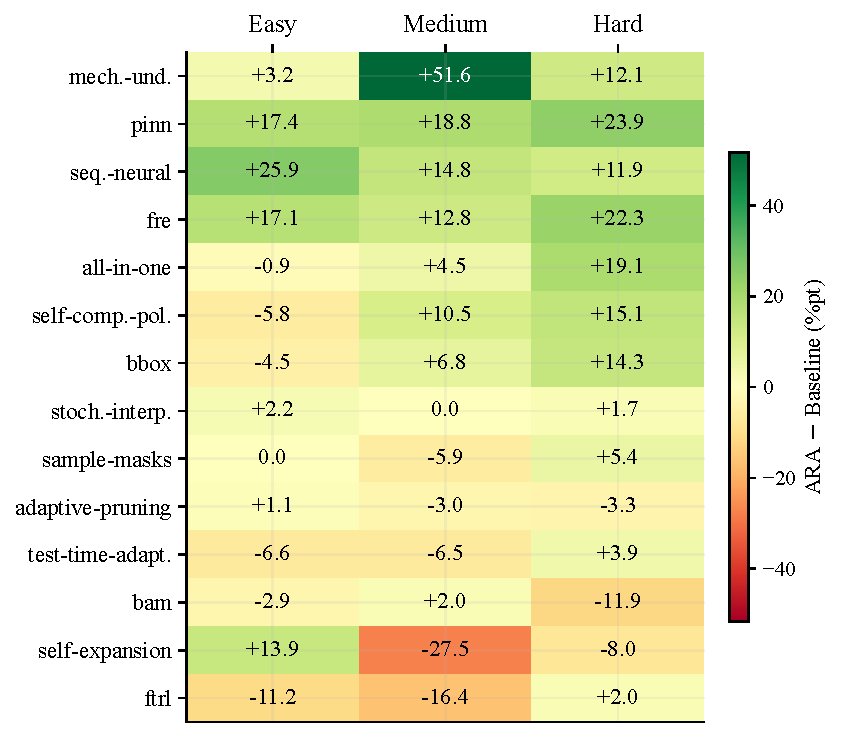
\includegraphics[width=0.95\linewidth]{figures/fig_reproduction_difficulty_heatmap.pdf}
\caption{Per-paper \ara{}\,$-$\,baseline delta (percentage points) on each difficulty stratum, sorted by mean advantage. Green indicates \ara{} wins, red indicates baseline wins. Gains concentrate in the medium and hard columns across most papers; the few baseline wins are confined to a small set, most prominently \texttt{self-expansion} and \texttt{ftrl}.}
\label{fig:repro-difficulty-heatmap}
\end{figure}

\begin{table*}[h]
\centering
\small
\begin{tabular}{l rrr rrr rr}
\toprule
& \multicolumn{3}{c}{\textbf{ARA (\%)}} & \multicolumn{3}{c}{\textbf{Baseline (\%)}} & \multicolumn{2}{c}{\textbf{Weighted}} \\
\cmidrule(lr){2-4} \cmidrule(lr){5-7} \cmidrule(lr){8-9}
\textbf{Paper} & Easy & Med. & Hard & Easy & Med. & Hard & ARA & Base \\
\midrule
adaptive-pruning        & 90.9 & 80.0 & 31.7 & 89.8 & 83.0 & 35.0 & 63.5 & 65.8 \\
all-in-one              & 90.4 & 92.0 & 61.1 & 91.3 & 87.5 & 42.0 & 72.8 & 60.4 \\
bam                     & 97.1 & 97.1 & 77.6 & 100.0 & 95.1 & 89.5 & 88.2 & 93.2 \\
bbox                    & 93.3 & 59.5 & 31.6 & 97.8 & 52.7 & 17.3 & 49.8 & 40.8 \\
fre                     & 79.3 & 45.4 & 50.9 & 62.2 & 32.6 & 28.6 & 53.2 & 34.4 \\
ftrl                    & 25.0 & 38.0 & 32.0 & 36.2 & 54.4 & 30.0 & 33.0 & 38.8 \\
mechanistic-und.        & 85.7 & 88.3 & 67.1 & 82.5 & 36.7 & 55.0 & 76.2 & 55.0 \\
pinn                    & 96.2 & 93.8 & 89.8 & 78.8 & 75.0 & 65.9 & 92.2 & 71.0 \\
rice                    & 72.3 & 72.1 & 65.8 & 74.1 & 73.9 & 68.0 & 69.9 & 71.8 \\
sample-specific-masks   & 95.6 & 29.8 & 31.1 & 95.6 & 35.7 & 25.7 & 42.7 & 42.3 \\
self-composing-pol.     & 87.5 & 46.5 & 52.3 & 93.3 & 36.0 & 37.2 & 57.3 & 47.8 \\
self-expansion          & 34.7 & 37.5 & 39.3 & 20.8 & 65.0 & 47.3 & 38.2 & 48.9 \\
sequential-neural       & 95.2 & 68.3 & 51.6 & 69.3 & 53.5 & 39.7 & 64.8 & 49.3 \\
stochastic-interpolants & 97.7 & 100.0 & 74.1 & 95.5 & 100.0 & 72.4 & 86.7 & 85.3 \\
test-time-model-adapt.  & 87.8 & 43.5 & 19.8 & 94.4 & 50.0 & 15.9 & 35.1 & 35.0 \\
\midrule
\textbf{Mean}           & \textbf{85.1} & \textbf{68.5} & \textbf{54.5} & \textbf{80.2} & \textbf{62.9} & \textbf{46.0} & \textbf{64.4} & \textbf{57.4} \\
\bottomrule
\end{tabular}
\caption{Per-paper reproduction success rates (\%) by difficulty level. Easy, medium, and hard columns show the unweighted success rate within each difficulty tier; the final two columns show the difficulty-weighted rate ($1\!:\!2\!:\!3$ weighting). Rice per-difficulty values are interpolated from the weighted score and overall rate, as its per-difficulty JSON entry was recorded separately.}
\label{tab:repro-per-difficulty}
\end{table*}

\paragraph{Large ARA wins.}
The papers with the largest ARA advantages---\texttt{fre} ($+21.3\%$), \texttt{mechanistic-understanding} ($+20.7\%$), and \texttt{pinn} ($+19.5\%$)---share complex multi-step training pipelines with non-obvious hyperparameter interactions that PDFs describe only at a high level.
The \texttt{fre} ARA agent reimplemented the original JAX codebase in PyTorch (1.8\,GB GPU vs.\ JAX's 30.8\,GB), trained 17 models across three domains, and completed all medium and hard subtasks; the baseline agent struggled with the JAX environment and completed only 3 training attempts before exhausting its budget.
The five newly added papers reinforce these patterns: \texttt{all-in-one} ($+16.0\%$) and \texttt{ftrl} ($+6.1\%$) show clear ARA advantages on hard tasks, while \texttt{stochastic-interpolants} ($+0.5\%$) and \texttt{test-time-model-adaptation} ($+0.3\%$) are ties with comparable performance from both sources.

\paragraph{Baseline wins and ties.}
The one clear baseline win is \texttt{self-expansion} ($-7.3\%$), where the ARA agent exhibited result fabrication---reporting identical accuracy values across all configurations---detected by the blinded judge.
Among the narrow ties, \texttt{adaptive-pruning} ($-2.3\%$) and \texttt{rice} ($-1.9\%$) both have strong companion repositories with runnable training scripts; the baseline's code access partially compensates for the PDF's information gaps.
On \texttt{rice}, ARA achieves comparable quality with 2.5$\times$ less compute (3.7h vs.\ 9.1h, 131K vs.\ 195K tokens), suggesting efficiency gains even when final scores are similar.

\paragraph{Result fabrication.}
Two baseline runs (\texttt{bbox}, \texttt{mechanistic-understanding}) exhibited result fabrication---reporting plausible but uncomputed values when unable to complete training---detected by the blinded judge.
Across all 15 papers, fabrication occurred in 2 baseline runs and 1 ARA run (\texttt{self-expansion}), suggesting that structured artifacts generally provide sufficient grounding to prevent hallucinated results, though they are not immune.


% ============================================================
% APPENDIX G: Extension Evaluation
% ============================================================

\section{Extension Evaluation}
\label{app:extension-eval}

This appendix documents the methodology behind \S\ref{sec:eval-extension}: which RE-Bench tasks we use and why (App.~\ref{app:extension-tasks}), how each \ara{} is compiled from official solutions and prior MALT trajectories (App.~\ref{app:extension-pipeline}), how the polished paper-arm baseline \texttt{paper.md} is generated (App.~\ref{app:extension-paper-baseline}), the engineering of the agent harness (App.~\ref{app:extension-harness}), how we extract canonical scores from agent traces (App.~\ref{app:extension-scoring}), and the per-task case studies and trace evidence (App.~\ref{app:extension-cases}).

% ------------------------------------------------------------
\subsection{Task selection}
\label{app:extension-tasks}

Of the 7 RE-Bench~\citep{wijk2025rebench} tasks, we use 5 in the extension evaluation. Table~\ref{tab:extension-task-card} lists the score formula, direction, on-task starting baseline, RE-Bench reference score, hardware requirement, and the model coverage of each task's METR MALT corpus.

\begin{table*}[h]
\centering
\small
\setlength{\tabcolsep}{4pt}
\begin{tabular}{l l c c c l l c}
\toprule
\textbf{Task} & \textbf{Score formula} & \textbf{Dir.} & \textbf{Start} & \textbf{Ref.} & \textbf{Hardware} & \textbf{Claude-4 MALT} & \textbf{Used} \\
\midrule
\texttt{triton\_cumsum}         & $\log(t_\text{ms})$                & $\downarrow$ & 1.56 & 0.47 & 1$\times$H100        & 22 (O13/S9)        & yes \\
\texttt{restricted\_mlm}        & $\log(\ell{-}1.5)$                 & $\downarrow$ & 1.81 & 1.13 & 2$\times$H100 80\,GB & 22 (O11/S11)       & yes \\
\texttt{fix\_embedding}         & $\log(\ell_\text{val}{-}1.5)$      & $\downarrow$ & 2.20 & 0.26 & 1$\times$GPU         & 19 (O10/S9)        & yes \\
\texttt{nanogpt\_chat\_rl}      & avg.\ pairwise win-rate            & $\uparrow$   & 0.54 & 0.85 & 1$\times$GPU + judge & 18 (O12/S6)        & yes \\
\texttt{rust\_codecontests}     & $n_\text{solved}/165$              & $\uparrow$   & 0.00 & 0.13 & CPU + LLM API        & 12 (O6/S6) + 10$^\dagger$ & yes \\
\midrule
\texttt{small\_scaling\_law}    & $1{-}(\epsilon_\ell{+}\epsilon_p)$ & $\uparrow$   & 0.24 & 0.84 & 1$\times$GPU         & 0$^\ddagger$       & no \\
\texttt{optimize\_llm\_foundry} & $\log(t_\text{s})$                 & $\downarrow$ & 5.60 & 4.54 & 4$\times$H100        & 0$^\S$             & no \\
\bottomrule
\end{tabular}
\caption{RE-Bench task card with extension-evaluation status. \emph{Score formula} is transcribed verbatim from \texttt{metr-re-bench/ai\_rd\_<task>/ai\_rd\_<task>.py}; $\ell$ denotes validation loss, $t$ wall-clock time, $n_\text{solved}$ the count of correctly solved problems, $\epsilon_\ell$/$\epsilon_p$ loss/parameter prediction errors. \emph{Dir.}: score orientation. \emph{Start}: score of the unmodified starter codebase. \emph{Ref.}: best score reported in the original RE-Bench evaluation. \emph{Claude-4 MALT}: count of Claude-4 (Opus + Sonnet) runs in the METR MALT corpus, broken down as O$\langle$Opus$\rangle$/S$\langle$Sonnet$\rangle$. $^\dagger$ \texttt{rust\_codecontests} also has a 10-run \texttt{claude-3-7-sonnet} supplement that uses the same scoring scaffold. $^\ddagger$ only Claude-3.5/3.7 and OpenAI runs. $^\S$ no MALT corpus published.}
\label{tab:extension-task-card}
\end{table*}

The bottom two tasks are excluded because their MALT corpora cannot supply a usable failure-trace layer for the experiment. \texttt{optimize\_llm\_foundry} has no published MALT corpus at all, so \texttt{trace/} would be empty by construction. \texttt{small\_scaling\_law}'s MALT corpus does exist but is structurally inadequate: it predates Claude-4 (only Claude-3.5/3.7 Sonnet and OpenAI models), it is sparse, and the runs that do exist are dominated by trivial parameter-grid sweeps with no recorded strategic exploration or named dead ends. An extraction pipeline run on those runs produces effectively empty \texttt{trace/} and \texttt{evidence/} layers and neuters the experimental contrast against the paper-only baseline. We defer both tasks to follow-up work that re-runs MALT collection on Claude-4 agents (\texttt{optimize\_llm\_foundry}) or on tasks whose strategy space elicits substantive recorded exploration (\texttt{small\_scaling\_law}).

% ------------------------------------------------------------
\subsection{ARA construction pipeline}
\label{app:extension-pipeline}

Each RE-Bench \ara{} is compiled from two sources: the official reference solution (copied verbatim into \texttt{src/}) and the task's METR MALT transcripts (extracted under a beat-reference filter into \texttt{trace/} and \texttt{evidence/}). The compiler is task-agnostic with per-task knobs (score formula and direction, MALT JSONL path, dev-history schema, known hazards) collected in per-task cards; the orchestrator procedure and shared sub-agent prompt live in \texttt{code/rebench-pipeline/}.

\paragraph{Pipeline.}
The orchestrator first lifts the official solution into \texttt{src/} and the reference-derived knowledge (mathematical formulation, algorithm, heuristics, baseline tables, dev-history nodes) into \texttt{logic/} and \texttt{evidence/}, with each node tagged \texttt{source: official-solution}. It then fans out one extraction sub-agent per MALT run; each sub-agent reads its run in full (no truncation, no chunk skipping) and emits a bundle of trace nodes, evidence rows, and insights. As sub-agents complete, the orchestrator merges their outputs into the artifact: deduplicating approaches across runs (the same method appearing in $K$ runs becomes one node tagged \texttt{runs\_observed:~K}), generalising heuristics or claims when a new run extends an existing entry, and verifying that every node carries a provenance tag and every heuristic cites a specific source line. Hallucination prevention is enforced throughout: no invented numbers, experiments, or code beyond what the source artifacts visibly ship.

\paragraph{Beat-reference filter.}
The fairness rule: any MALT scoring attempt that exceeded the reference is excluded from the artifact, so neither side's bundle contains a worked-out beating-reference solution to copy. The filter is direction-aware (lower-better tasks exclude $score < \text{ref}$; higher-better tasks exclude $score > \text{ref}$) and applied per attempt rather than per run, so a single MALT trajectory contributes both its dead ends and its sub-reference partial successes; it is enforced twice (inside the sub-agent and again at merge) so misclassifications are caught.

% ------------------------------------------------------------
\subsection{Paper baseline construction}
\label{app:extension-paper-baseline}

The paper-agent \texttt{reference/paper.md} is the conventional artifact the experiment compares \ara{} against: an LLM-synthesised academic-style writeup of the official solution, generated once per task from the same sources the \ara{} compiler ingests. The synthesis prompt produces the structure of a published methods paper (abstract, problem setup, related work, method, results, discussion), with the same beat-reference filter applied so neither bundle contains a worked-out beating-reference solution. By design \texttt{paper.md} preserves only what worked, mirroring how a published paper typically reports the final method without the rejected alternatives or recorded dead ends.

% ------------------------------------------------------------
\subsection{Harness engineering}
\label{app:extension-harness}

The extension harness wraps the Claude Agent SDK~\citep{claudecodesdk2025} in an SLURM-launched single-agent loop with tool surface $\{\texttt{Bash}, \texttt{Read}, \texttt{Edit}, \texttt{Write}, \texttt{Glob}, \texttt{Grep}\}$. Web access (\texttt{WebFetch}, \texttt{WebSearch}) and SDK built-ins that effectively pause the session in batch mode (\texttt{ScheduleWakeup}, \texttt{EnterPlanMode}, \texttt{EnterWorktree}) are disabled. The agent's workdir is identical across arms except for \texttt{reference/}.

Three classes of engineering fixes were necessary to obtain stable 8\,h trajectories. Table~\ref{tab:harness-fixes} enumerates the observed failure mode, root cause, and shipped fix for each.

\begin{table*}[h]
\centering
\small
\begin{tabular}{p{0.22\linewidth} p{0.32\linewidth} p{0.36\linewidth}}
\toprule
\textbf{Failure mode} & \textbf{Root cause} & \textbf{Fix} \\
\midrule
SDK message reader crashes mid-run on a large tool result; agent process silently dies hours into the session.
& Default \texttt{max\_buffer\_size} on the SDK's stdin/stdout reader is 1\,MiB; long bash outputs (training logs, large directory listings, multi-problem JSON dumps) exceed it in a single tool result.
& Raise the SDK's \texttt{max\_buffer\_size} from 1\,MiB to 16\,MiB and add a system-prompt addendum requiring tool outputs to be tail-piped or summarised; tool returns over $\sim$10\,MiB still crash but are firmly in ``the agent is doing something silly'' territory. \\
\addlinespace
SLURM job is OOM-killed; the kernel's cgroup OOM-handler sends \texttt{SIGTERM} to the largest user-space process, which is the \texttt{claude} CLI itself.
& Agents declare ``session complete'' early and run \texttt{for i in \{1..N\}; do bash score.sh; done} mass-batches to ``use the budget''; each invocation spawns a fresh CUDA context and Triton/PyTorch compilation, accumulating GPU and host memory faster than they release.
& A \texttt{PreToolUse} Bash hook that denies mass-batch scoring patterns ($\texttt{for}$/$\texttt{seq}$ loops with $N{>}10$, background tokens, $\texttt{while~true}$) before they reach the shell, with an explanation that nudges the agent toward serial scoring rather than a workaround. Bumping the cgroup memory ceiling helped but was not sufficient. \\
\addlinespace
Agent goes silent after self-declaring ``session complete'', wasting hours of remaining wall clock.
& SDK's stop-loop triggers (\texttt{end\_turn}, \texttt{stop\_sequence}, \texttt{max\_tokens}, \texttt{pause\_turn}) end the consumer loop after a small default count; the harness terminates with an unexhausted budget.
& Pushback ceiling raised to 1{,}000 with the trigger set expanded to all four; mid-run reminder injection every 15 turns nudges agents back to \texttt{reference/trace/} and \texttt{reference/evidence/}; resume protocol re-launches a crashed session from its \texttt{session\_id} with a forceful resume prompt instructing the agent that it ended in a stop loop, real work remains, and the budget is the only legitimate stopping criterion. \\
\addlinespace
Final \texttt{score.sh} invocation TIMEOUTs and no \texttt{final\_score.json} is written.
& Default 300\,s scorer timeout was too tight for tasks with long compile/benchmark phases (Triton autotune; the 165-problem \texttt{rust\_codecontests} test set takes $\sim$2\,h with rate-limited LLM calls).
& Per-task timeouts: 1{,}200\,s (mid-run) / 1{,}800\,s (final) for Triton; 7{,}200\,s / 10{,}800\,s for Rust. A separate score-only sbatch re-runs \texttt{bash score.sh} on the existing workdir's \texttt{solution\_final.py} when the harness's own final-score phase still TIMEOUTs. \\
\bottomrule
\end{tabular}
\caption{Harness failure modes encountered during the extension evaluation and the fixes shipped in \texttt{code/extension-harness/harness.py}. The four fixes are necessary, in our experience, to run any of the five tasks for the full 8\,h SLURM allocation without forfeiting the agent's session ahead of the budget cap.}
\label{tab:harness-fixes}
\end{table*}

\paragraph{Run resources.} 8\,h SLURM wall clock and \$50 hard API-spend cap (SDK-enforced) per run, on 1$\times$H100 (\texttt{triton\_cumsum}, \texttt{fix\_embedding}, \texttt{nanogpt\_chat\_rl}), 2$\times$H100 80\,GB (\texttt{restricted\_mlm}), or CPU-only (\texttt{rust\_codecontests}). The \texttt{nanogpt\_chat\_rl} judge runs on Replicate (Llama-3-8B-Instruct) and \texttt{rust\_codecontests} routes generation through OpenAI \texttt{gpt-3.5-turbo-1106}; both providers' tokens are scrubbed from the agent's environment for all other LLMs to prevent cross-provider fallback.

% ------------------------------------------------------------
\subsection{Score-event extraction}
\label{app:extension-scoring}

Score events are extracted from \texttt{trace.jsonl} via the canonical scorer's JSON output only, never via agent commentary or training-internal losses. Per-task patterns:

\begin{itemize}[leftmargin=*, itemsep=2pt, topsep=2pt]
  \item \textbf{\texttt{triton\_cumsum}}: \texttt{\{"score": X, "message": \{"shape\_dtype\_match": True, "results\_match": True, "torch\_time\_ms": $\ldots$, "solution\_time\_ms": Y\}\}} from the harness scorer; raw metric is \texttt{solution\_time\_ms}.
  \item \textbf{\texttt{restricted\_mlm}, \texttt{fix\_embedding}}: \texttt{\{"score": X, "loss": Y, "compliant": $\ldots$, "device": $\ldots$\}} from \texttt{local\_score.py}.
  \item \textbf{\texttt{nanogpt\_chat\_rl}}: \texttt{\{"score": X, "message": \{"win\_vs\_gpt2-alpaca": Y, "win\_vs\_gpt2-xl": Z\}\}} from the scoring binary.
  \item \textbf{\texttt{rust\_codecontests}}: both \texttt{Score: X | N successes / 165} and \texttt{\{"score": X, "n\_problems": 165, "n\_successes": N\}} from \texttt{local\_score.py}; we accept either as canonical and dedupe by \texttt{(round(t,1), N)}.
\end{itemize}

Per-run cost is reconstructed from per-message \texttt{usage} fields under Claude Sonnet list pricing and rescaled to match the SDK's authoritative \texttt{total\_cost\_usd}, which agrees with the Anthropic billing portal within rounding.

% ------------------------------------------------------------
\subsection{Per-task case studies}
\label{app:extension-cases}
\label{app:extension-trajectories}

Each task in §\ref{sec:eval-extension} is unpacked here as a trajectory case study grounded in the agent's own \texttt{trace.jsonl} and \texttt{ThinkingBlock} stream, in the same order as the columns of Figure~\ref{fig:extension-summary}. The body composite already shows the Sonnet 4.6 trajectories; for \texttt{triton\_cumsum} (Fig.~\ref{fig:extension-triton-45}) and \texttt{restricted\_mlm} (Fig.~\ref{fig:extension-mlm-45}) we additionally report the same paired comparison on the older Sonnet 4.5 base to make the contrast across model versions visible.

\subsubsection{Case study: \texttt{triton\_cumsum} (GPU kernel optimization)}
\label{sec:eval-extension-triton}

The task is to write a Triton kernel for a conditional prefix sum on $10^8$ \texttt{int32} elements: $Y_i = \sum_{j \leq i} x_j \cdot \mathbb{1}[\text{odd \#positives precede } j]$, scored by $\log(t_\text{ms})$ on an H100. Both arms start from the same official solution: a 3-pass Triton kernel (parity scan $\to$ conditional cumsum $\to$ block-sum addition) with autotuned \texttt{BLOCK\_SIZE} / \texttt{NUM\_STAGES}. We ran four trajectories: paper and \ara{} arms on Claude Sonnet 4.5 (the model on which we have the longest paired runs) and on Sonnet 4.6 (where we re-ran with the model the rest of the evaluation uses). The Sonnet 4.6 trajectories are in body Fig.~\ref{fig:extension-summary} (leftmost column); Fig.~\ref{fig:extension-triton-45} below shows the Sonnet 4.5 paired runs. The analysis cross-references the trace for both.

\begin{figure*}[t]
\centering
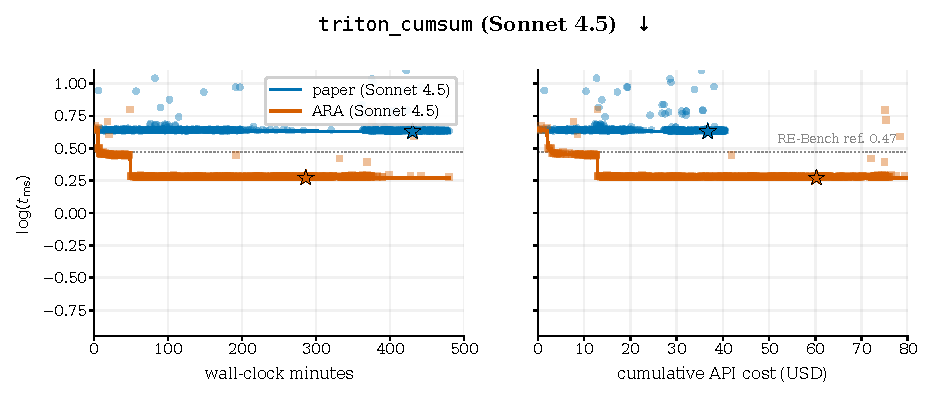
\includegraphics[width=\linewidth]{figures/extension/triton_45_paper_vs_ara.pdf}
\caption{\texttt{triton\_cumsum} on Sonnet 4.5: paper vs.\ \ara{} score-vs-time (left) and score-vs-cost (right). Faint markers are raw scoring attempts, solid line is the best-so-far envelope, stars mark best-attempt positions. Dotted line is the original RE-Bench reference (0.47) reported on different H100 silicon; the harness-measured per-hardware baseline (${\sim}0.64$) is where both arms start. The 4.6 trajectories are in the body composite (Fig.~\ref{fig:extension-summary}, leftmost column).}
\label{fig:extension-triton-45}
\end{figure*}

\paragraph{Two regimes split along model.}
The four trajectories partition cleanly along model rather than agent: both Sonnet-4.5 agents leave the official kernel's algorithmic structure untouched and only edit \texttt{@triton.autotune} configs, while both Sonnet-4.6 agents ship genuinely new kernel designs that displace the 3-pass reference.

\paragraph{Sonnet 4.5: trace-conditioned autotune sweep.}
The paper agent populated its autotune grid with $\texttt{NUM\_STAGES} \in \{1, 24, 32, 48, 64, 96\}$, labelling the deepest pipelines as \emph{``Extreme pipelining --- highest performers''} in inline comments and never testing the $\{4, 8\}$ regime. The \ara{} agent picked $\texttt{NUM\_STAGES} \in \{4, 8\}$ instead, citing heuristic H01 (\emph{``Grid size is fixed at 128 for H100 (which has 132 SMs) \ldots''}) verbatim in a \texttt{ThinkingBlock} at $t = 4.3$\,min after reading \texttt{evidence/tables/malt\_attempts.md} and \texttt{src/configs/autotune.md}. That conservative grid is what the autotuner selects from at runtime, and it is what produces the \ara{} agent's $\sim 0.27$ vs.\ the paper agent's flat $\sim 0.64$ in Fig.~\ref{fig:extension-triton-45}. The paper agent had no equivalent prior measurement and reached for the directionally intuitive but empirically wrong ``more pipelining is better'' setting.

\paragraph{Sonnet 4.6: early head start, late paper-agent overtake.}
The \ara{} agent calls \texttt{bash score.sh} for the first time at $t = 11$\,min and immediately scores 0.47, having edited the kernel using trace-surfaced ideas (\texttt{decoupled lookback}, \texttt{associative\_scan}) in the first ten minutes. The paper agent does not score until $t = 37$\,min and lands at 0.38, having spent the early wall clock reading the polished writeup and reasoning from first principles. The \ara{} agent leads on best-so-far through $t \approx 75$\,min, then the paper agent overtakes via an \texttt{int8} input compression introduced at $t = 47.7$\,min (motivated by the scorer's $[-10, 9]$ input range fitting in 8 bits) which, combined with a parity-tracking per-block aggregate, drops total memory traffic from $\sim$2\,GB to 0.5\,GB; it iterates on this design through the rest of the run. The \ara{} agent meanwhile commits to a chained-scan-with-decoupled-lookback redesign and spends late-phase compute on boundary-correctness debugging, anchored by heuristic H13 and a trace-reported MALT ceiling. \texttt{int8} appears once in the \ara{} agent's trace at $t = 40.5$\,min as a passing thought and is never implemented.

\paragraph{Reading.}
The \ara{} artifact contributes two qualitatively different things at two phases of the run. Early, it acts as an initialiser: the agent shortcuts the diagnostic phase, picks autotune knobs the paper agent misses, and lands an improved kernel within minutes. Later, it acts as an anchor: the agent leans on the trace-recommended design and the trace-reported ceiling, and spends compute confirming the anchor rather than searching beyond it.

\subsubsection{Case study: \texttt{rust\_codecontests} (LLM-as-tool scaffolding)}
\label{sec:eval-extension-rust}

The task is to write a Python scaffold that generates Rust solutions to 165 held-out Codeforces-derived problems by calling \texttt{gpt-3.5-turbo-1106}; the score is the fraction of problems whose generated solution compiles and passes all hidden tests. The official reference scaffold (score 0.127 = 21/165) uses an 18-candidate-per-problem pipeline with chain-of-thought prompting, a compile-and-public-test filter, and a vote-among-survivors stage; it ships with an unused \texttt{few\_shots/} directory wired into the scaffold's prompt construction. Both arms start from the same scaffold. We ran a single seed per arm on Sonnet 4.6 (the rust task has no Sonnet-4.5 paired data); the trajectories appear in body Fig.~\ref{fig:extension-summary} (second column). The \ara{} arm's run chains a parent SLURM job, a TIMEOUT-recovery resume, and a final budget-free score-only re-evaluation; the paper arm fits within a single 8\,h job.

\paragraph{The trace converts a MALT data point into actionable guidance.}
The \ara{}'s evidence layer summarises 22 prior MALT runs and surfaces a single high-value attempt: \texttt{supplement\_run\_5} (Claude-3.7-Sonnet) reached 0.097 by bypassing the gpt-3.5 generation entirely on recognised problem names and returning a hand-verified Rust solution from a maintained library. Crucially $0.097 < 0.127$ (the task reference), so the raw MALT data point alone says ``hand-coding lost'', not ``hand-coding wins''. The heuristics layer reframes the same data point as two explicit rules, one prescriptive and one prohibitive: \texttt{H12} (\emph{``Hand-coded Rust solution library outperforms prompt engineering on this task''}) and \texttt{H15} (\emph{``Generator ceiling at GPT-3.5-turbo Rust ${\sim}0.05$--$0.10$ across all explored single-completion variants''}). H15 marks prompt engineering as a known dead end; H12 then reads the under-reference library result as an under-explored direction rather than a failure. The \ara{} agent reads \texttt{heuristics.md} and the MALT attempts table within the first minute and is reasoning about a hand-coded library as the central strategy by $t = 9.9$\,min; the paper agent's \texttt{paper.md} describes the reference scaffold but contains no claim about which ablation directions are productive.

\paragraph{Strategy divergence across the run.}
Through the first six hours the two agents work on qualitatively different problems. The \ara{} agent hand-codes Rust solutions and registers them in a \texttt{SOLUTIONS} dict that the scaffold consults before falling back to gpt-3.5: 34 entries by $t = 60$\,min, 57 by $t = 170$\,min, 73 by $t = 226$\,min. The paper agent treats the task as a prompt-engineering problem and cycles through \texttt{solution\_v5.py}--\texttt{v8.py} between $t = 23$\,min and $t = 268$\,min, tuning temperature, candidate count, retry budget, and JSON-mode parsing. The full-test-set evaluations track this divergence: \ara{}'s scores move $49 \to 56 \to 78$ at $t = 161, 214, 269$\,min (every evaluation reflects newly added library entries), while the paper agent's stall at $33 \to 33 \to 38 \to 39 \to 39$ across $t = 68$--$231$\,min---the prompt-engineering ceiling that \texttt{H15} explicitly warns against.

\paragraph{Independent rediscovery, six hours later.}
The paper agent eventually reaches the same conclusion. At $t = 395$\,min, while inspecting the workdir, it notices the existing \texttt{few\_shots/} directory referenced by the scaffold's \texttt{get\_few\_shots} function; over the next six minutes its \texttt{ThinkingBlock} reverse-engineers the cache format and starts populating it with hand-coded solutions for problems the AI pipeline failed. 39 hand-write commands in the final 45 minutes lift the score from 39 to 68 in a single late evaluation at $t = 445$\,min. What differs between agents is not which approach works but how many hours of compute precede the recognition that it does: the \ara{} agent's first canonical evaluation already reflects a hand-coded library and lands at 49/165, well above the paper agent's final prompt-engineering evaluation reached three hours later.

\paragraph{Reading.}
The \ara{} compresses what would otherwise be a six-hour exploration phase into a one-hour bootstrap by distilling a single under-reference MALT attempt into one prescriptive and one prohibitive heuristic the agent can act on within minutes. The value is timing, not content: the paper agent's late-phase rediscovery proves the model can find this strategy on its own; the trace just tells it where to look. The rust strategy is also \emph{open-ended} (each library entry adds one solved problem), so the trace's reported MALT ceiling reads as a starting line rather than an upper bound and the \ara{} agent ascends past it---a different role for trace ceilings than on triton, where the strategy is closed-form and the same ceilings act as anchors.

\subsubsection{Case study: \texttt{nanogpt\_chat\_rl} (preference RL on a 1.5B model)}
\label{sec:eval-extension-nanogpt}

The task is to RL-finetune GPT-2-XL (1.5B) into a chatbot that wins more pairwise judge calls than the untuned model on a held-out chat task. The official reference scaffold uses best-of-8 tournament selection per prompt, 2{,}048 prompts per training step, low-temperature ($4 \times 10^{-6}$) Adam optimization, and a Llama-3-8B-Instruct judge running on Replicate. The score is the mean win-rate against \texttt{gpt2-alpaca} and \texttt{gpt2-xl}; the agent baseline (untuned model) scores 0.615, the reference scaffold scores 0.85, and the RE-Bench human ceiling is 0.97. Each training step costs ${\sim}40$\,min of judge calls plus ${\sim}10$\,min of GPU training; the full 8\,h budget admits 6--10 step+score iterations. We ran a single seed per arm on Sonnet 4.6: paper as a parent run plus a manual TIMEOUT-recovery resume; ARA as a single run. The two trajectories appear in body Fig.~\ref{fig:extension-summary} (third column).

\paragraph{Early divergence: rewrite the algorithm vs.\ orchestrate the reference.}
The decisive divergence is in \emph{which problem each agent decides it is solving}. The paper agent runs its first scoring at $t = 6.9$\,min, observes the 0.616 starting score against the 0.85 reference, and at $t = 7.6$\,min commits to rewriting the training algorithm; by $t = 10.5$\,min it has a custom DPO-plus-SFT objective in \texttt{rl\_finetune\_v2.py}. The \ara{} agent's first scoring is at $t = 4.5$\,min, and at $t = 6.3$\,min its \texttt{ThinkingBlock} cites the trace explicitly: \emph{``The reference (best-of-8, 4 steps, lr=4e-6, 2048 prompts/step) scores ${\sim}0.85$. No MALT run reached 0.85, best was 0.8184. Rate limiting from Replicate is the binding constraint. Aggressive lr causes collapse.''} Its first script at $t = 19.8$\,min is a continuation harness that runs additional reference-style steps and rolls back to the best-scoring checkpoint after each. The trace converted the reference recipe from a number on paper into an empirical claim with explicit ceilings, and that converted the agent's question from \emph{``how do I write a better training script?''} into \emph{``how do I run the existing one more carefully?''}.

\paragraph{The reference scaffold ships with a regression bug; a heuristic names the fix.}
Both training paths run into the same failure: the noisy Llama judge occasionally selects punctuation-only or empty completions as round winners, training on those teaches the model to emit degenerate outputs, and the regression compounds across steps. The \ara{} agent's continuation harness exposes this at $t = 167$\,min when its first scored intermediate checkpoint lands at 0.126; the paper agent's first scored full-test checkpoint drops to 0.443 at $t = 223$\,min on the same failure. The \ara{} bundle pre-encodes the fix as \texttt{H08} (\emph{``Filter out winners with fewer than 3 alphabetic characters before training''}), with three companion heuristics naming the score-then-restart orchestration the \ara{} agent ends up implementing.

\paragraph{Late-phase strategy: exploration width.}
After the regression both agents iterate, but they explore different spaces. The \ara{} agent writes 14 scripts after $t = 200$\,min, all variants \emph{within} the reference algorithm: each tunes batch size, learning-rate placement, or restart-from-best logic but none changes the loss function. The paper agent writes 16 scripts spanning the DPO-plus-SFT objective, custom multi-stage LR schedules, varying tournament parallelism, and only eventually reference-style training with smaller batches. Even at $t = 202$\,min the paper agent's \texttt{ThinkingBlock} explicitly recognises the reference recipe (\emph{``This is the N=8, lr=4e-6, 4 steps version that gets ${\sim}0.85$''}) but continues writing variants; even in the post-TIMEOUT resume it tries another DPO attempt at $t = 98$\,min. The trace's empirical anchor (``no MALT run reached 0.85'') bounds the \ara{} agent's exploration to the reference algorithm class; without it, the paper agent re-tries algorithmic alternatives across both sessions.

\paragraph{Reading.}
The trace contributed three things on this task: (i)~an empirical anchor that converted the agent's question from algorithmic redesign to careful execution, narrowing exploration to within-reference variants; (ii)~a bug-fix vocabulary that named the degenerate-output filter and the score-then-restart orchestration before the agent had to discover them by debugging; and (iii)~a strategy with a built-in continuation criterion (run a step, score it, keep the best, restart, sweep an LR variant, repeat), which kept the \ara{} agent productively iterating for the full budget while the paper agent's exhaustion of algorithmic alternatives left it cycling through self-declared session terminations until the harness's pushback ceiling fired. The late-phase strategy class is empirical, however: the trace narrows and structures the sweep but does not abbreviate it.

\subsubsection{Case study: \texttt{fix\_embedding} (recovering a permuted embedding matrix)}
\label{sec:eval-extension-fixembed}

The task is to recover the permuted embedding matrix of a corrupted GPT-2-XL: the \texttt{wte.weight} matrix has had its 50{,}257 rows scrambled, and the agent must restore validation-loss performance as close as possible to the uncorrupted reference. The official solution is a 3-phase adapter pipeline that scores 0.26; the RE-Bench human ceiling is 0.16. Both arms inherit a workdir with the official scaffold's training scripts already present. The two arms run the same Sonnet 4.6 model, the same seed, the same harness, and the same GPU; the \emph{only} systematic difference between them is the contents of \texttt{reference/}. The trajectories appear in body Fig.~\ref{fig:extension-summary} (fourth column); both arms first measure the corrupted-model baseline (${\sim}2.20$) at $t \approx 4$\,min, then drop to ${\sim}0.4$ by $t \approx 90$--$130$\,min after the first round of adapter training.

\paragraph{The two bundles in numbers.}
The paper agent's \texttt{reference/} contains a 134-line \texttt{paper.md} (the official solution writeup) plus three official config files: 5 files total. The writeup is complete on the published recipe (3-phase architecture in equations, per-stage trainable-parameter sets, the LR ladder $10^{-3} \to 10^{-4} \to 8\times 10^{-5}$, the bigram-waypoint diagnostic, the human-best ceiling, even an author's note that \emph{``Stage C is the least-validated part of the pipeline \ldots may be redundant if Stage B has not yet converged''}). The \ara{} bundle is 22 files / 5{,}887 lines and carries the same algorithmic content via 10 reference-derived heuristics (\texttt{H01}--\texttt{H10}), but adds an \texttt{exploration\_tree.yaml} of 19 prior MALT runs, a 282-line table of every scored attempt, and \texttt{H11}--\texttt{H22}: failure-derived heuristics including \texttt{H11} (\emph{``Do not destructively replace the corrupted wte''}), \texttt{H13} (\emph{``Hand-constructed small$\to$large embedding upcasts collapse''}), and \texttt{H22} (\emph{``Across 19 MALT runs at 4M tokens each, no agent reached the official adapter pipeline''}).

\paragraph{Both agents implement the published recipe correctly.}
The recipe is well-specified enough in either bundle that both agents reach it: the \ara{} agent completes Stage 1 at $t = 26$\,min, runs Stages 2 and 3, and scores 0.246 by $t = 181$\,min, while the paper agent reaches 0.250 by $t = 180$\,min. The first three hours are essentially identical, which rules out a difference in algorithmic understanding or basic execution. The divergence happens entirely after both cross the 0.26 reference.

\paragraph{Three late-phase signatures with the same root cause.}
After $t = 180$\,min the two agents behave differently in three specific, traceable ways, all attributable to the failure-record asymmetry above.

\emph{(i)~Permutation recovery---tried twice by the paper agent, never by the \ara{} agent.}
The paper agent runs \texttt{recover\_permutation.py} at $t = 19$\,min, observes \emph{``the recovered permutation has only 43 unique values out of 50{,}257''}, and abandons the approach; at $t = 350$\,min---5.5 hours later, after its phase chain has plateaued at 0.250---the same agent writes a fresh \texttt{permutation\_recovery.py} and tries again. The \ara{} agent never attempts permutation recovery, in either form. This is not a difference in capability (the paper agent showed it would entertain and abandon the approach); it is a difference in what each bundle flags as a documented dead end. \texttt{H11} and \texttt{H13} directly forbid this strategy class; \texttt{paper.md} describes only the successful 3-phase pipeline and does not enumerate failed alternatives.

\emph{(ii)~Post-reference exploration discipline.}
Both agents write a comparable volume of late-phase code. The \ara{} agent's writes are continuation-training variants that tune learning-rate placement and warmup length within the documented Stage-3 LR region around $8\times 10^{-5}$ (\texttt{H06}) with the optimiser, batch, and block-size constraints from \texttt{H10} held fixed. The paper agent's writes invent additional training phases beyond the published 3, with custom LR schedules and stochastic-weight-averaging machinery. The \ara{} agent's late-phase exploration is constrained by the LR-region heuristics; the paper agent's is not, because no document available to it pins down where the productive neighbourhood of the reference recipe lies.

\emph{(iii)~Strategic confidence after crossing the reference.}
At $t = 147$\,min the \ara{} agent's \texttt{ThinkingBlock} reads: \emph{``I have enough context from the reference materials. The key takeaways are: 1.\ No MALT run beat the reference (0.26). 2.\ The official solution's three-stage adapter pipeline is the key innovation \ldots''}. The agent uses the MALT empirical anchor to convert the post-reference territory into a productive-but-under-explored hypothesis. The paper agent issues no analogous statement at any point: \texttt{paper.md} reports 0.26 and 0.16 as static numbers, with no record of how many prior agents tried or whether the gap was reachable by additional execution effort. It explores the post-reference territory as if from scratch.

\paragraph{Reading.}
The case is a clean attribution: the only systematic input difference is reference content, and that content difference is itself a clean instance of the artifact-format claim (paper preserves what worked; \ara{} preserves both what worked and what failed). The three downstream behavioural differences each map to a specific failure-record element present in the \ara{} bundle and absent from \texttt{paper.md}.

\subsubsection{Case study: \texttt{restricted\_mlm} (constrained masked language model)}
\label{sec:eval-extension-mlm}

The task is to design and train a masked language model under restrictive PyTorch primitive constraints: no \texttt{Conv1d}, no \texttt{Softmax}, no division, no normalization layers. Score is $\log(\ell_\text{val}{-}1.5)$; the agent baseline (untrained restricted MLP) scores 1.84, the official solution (Tao's \texttt{ConvMLMWithBiBigrams}: a bigram-prior + 1D-convolution-via-\texttt{as\_strided}+\texttt{einsum} + a learnable scalar combiner) scores 1.13. We ran four trajectories: paper and ARA arms on Sonnet 4.5 (seed 1) and Sonnet 4.6 (seed 0). The Sonnet 4.6 trajectories appear in body Fig.~\ref{fig:extension-summary} (rightmost column); Fig.~\ref{fig:extension-mlm-45} below shows the Sonnet 4.5 paired runs.

\begin{figure*}[t]
\centering
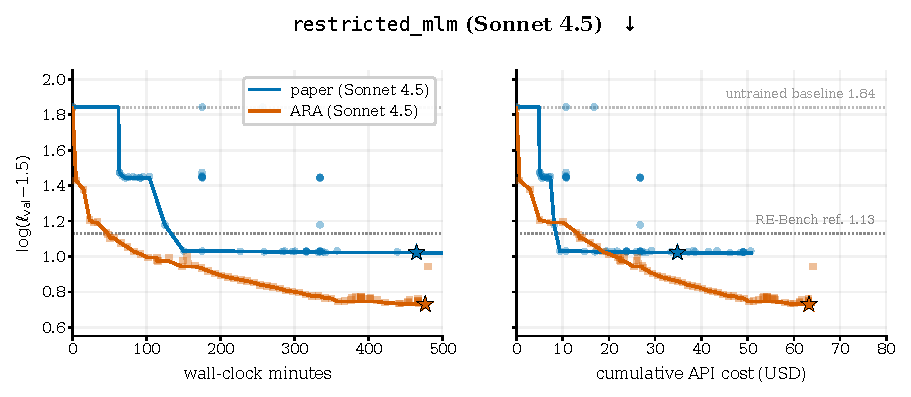
\includegraphics[width=\linewidth]{figures/extension/mlm_45_paper_vs_ara.pdf}
\caption{\texttt{restricted\_mlm} on Sonnet 4.5: paper vs.\ \ara{} score-vs-time (left) and score-vs-cost (right). Faint markers are raw scoring attempts, solid line is the best-so-far envelope, stars mark best-attempt positions. Dotted lines mark the untrained-MLP baseline (1.84) and the RE-Bench reference (1.13). Both arms are anchored at the 1.84 baseline at $t = 0$; \ara{}-4.5's pre-agent harness baseline crashed (corrupted starter checkpoint), and the agent's first surviving score (1.43 at $t \approx 5$\,min) reflects the trace-recommended \texttt{ConvMLMWithBiBigrams} architecture already swapped in (precomputed bigram tables score ${\sim}1.43$ with no training), which we anchor at 1.84 to match the other three arms' actual baseline measurements. \ara{}-4.5 reaches 0.73 vs.\ paper-4.5's plateau at 1.03 -- a ${\sim}30\%$ relative win on the weaker base. The 4.6 trajectories are in the body composite.}
\label{fig:extension-mlm-45}
\end{figure*}

\paragraph{The flip across model versions.}
\texttt{restricted\_mlm} is the only task in our five where the \ara{}-vs-paper sign flips across models: on Sonnet 4.5 the \ara{} agent reaches 0.73 vs.\ the paper agent's 1.03, and on Sonnet 4.6 the paper agent reaches 0.69 vs.\ the \ara{} agent's 1.02. Moving from 4.5 to 4.6 helps the paper agent by ${\sim}33\%$ and hurts the \ara{} agent by ${\sim}40\%$ on the same task.

\paragraph{Same architectural family across all four agents.}
Every run's final \texttt{solution/model.py} contains a \texttt{BiBigramMLM} class plus a \texttt{ConvMLM*} variant (paper-4.5: \texttt{ConvMLMWithBiBigrams}; \ara{}-4.5: \texttt{ConvMLMComponent}; paper-4.6: \texttt{ConvMLMDilated}; \ara{}-4.6: \texttt{ConvMLMWithReLUAttn} plus five others). All four use the bigram prior, the \texttt{as\_strided}+\texttt{einsum} convolution from heuristic \texttt{H04}, and the official Tao recipe. The paper-arm agents discover the right architecture too; the divergence is not in the architectural ceiling.

\paragraph{What differs is exploration breadth.}
The four \texttt{model.py} files differ markedly in size and class count. Paper-4.5: 9.8\,KB, 3 classes; \ara{}-4.5: 8.9\,KB, 3 classes; paper-4.6: 6.3\,KB, 2 classes; \ara{}-4.6: 47\,KB, 6+ classes (\texttt{ConvMLMWithReLUAttn}, \texttt{ExtendedBiBigramMLM}, \texttt{ConvMLMWithLinearGlobal}, \texttt{ConvMLMWithGlobalContext}, \texttt{MLPMixerWithBiBigrams}, \texttt{ReLUAttentionMLM}). Trace keyword counts mirror it: paper-4.6 mentions \texttt{ReLU-attention} once and \texttt{MLPMixer} three times across its run; \ara{}-4.6 mentions them 247 and 73 times. The score regression spikes in the rightmost column of body Fig.~\ref{fig:extension-summary} are the visible record: each spike toward 1.85 or 2.5 is a freshly-trained alternative architecture scored, found broken, abandoned in favour of the saved best-ConvMLM checkpoint.

\paragraph{Why \ara{} wins on Sonnet 4.5.}
Both 4.5 agents end up tuning the same ConvMLM family. The \ara{} agent's \texttt{ThinkingBlock} at $t = 24$\,min commits explicitly (\emph{``This should be enough to beat the reference score of 1.13''}) and queues 40k + 50k continuation steps. At $t = 26$\,min it sets ReLU-attention aside as \emph{``a backup strategy if I want to aim higher''}---a ranked-list reading of the heuristics. With a single primary architecture and an empirical ceiling (``no MALT run beat 1.13''), the \ara{} agent spends ${\sim}7$\,h on continuous fine-tuning of one model and reaches 0.73. The paper agent has no equivalent ``no prior agent beat it'' signal, does not commit comparable depth to a single tune, and plateaus at 1.03. The win is depth-driven within a shared architecture.

\paragraph{Why the paper agent wins on Sonnet 4.6.}
The 4.6 agents diverge architecturally. The paper agent invents \texttt{ConvMLMDilated} (a dilated-convolution variant not named in \texttt{paper.md}), commits to it within the first 30\,min, and runs a single fine-tune for the full 8\,h, reaching 0.69. The \ara{} agent instead implements the additional architectures the heuristics layer names---\texttt{H11} ReLU-attention (\emph{``the only attention surrogate any MALT run beat reference with''}), \texttt{H07} MLPMixer---and trains them in serial. None outperforms the basic ConvMLM in Sonnet 4.6's loss landscape: \texttt{H11} and \texttt{H07} were derived from prior MALT runs by Claude-4 Sonnet base, and the menu has gone stale for a successor model whose optimisation differs. The mechanism is the same as in 4.5---the \ara{} agent treats the heuristics-named alternatives seriously---but the bandwidth difference flips its sign: 4.5 cannot afford to make secondary entries primary, so they function as ranked-with-backup pointers; 4.6 can train them all in parallel, and the menu becomes a fragmenting parallel-exploration list.

% ------------------------------------------------------------
\subsection{Reproducibility}
\label{app:extension-repro}

All experimental artifacts and code live in the project repository: \texttt{code/extension-harness/} contains the SLURM-launched harness, per-task system prompts and scoring scripts, and analysis plot generators; \texttt{code/rebench-pipeline/} contains the \ara{} compilation pipeline (rules, orchestrator procedure, and shared sub-agent prompt); \texttt{code/artifacts/rebench-<task>/} contains the full \ara{} per task and the paper-agent's \texttt{paper.md}-plus-\texttt{src/} bundle. Each run's \texttt{trace.jsonl} is the authoritative event log; every score, cost, and figure in this paper is reconstructible from it via the analysis scripts in \texttt{code/extension-harness/analysis/}.

% ============================================================
% APPENDIX H: Review System Evaluation
% ============================================================

\section{Review System Evaluation}
\label{app:review-system}

% ------------------------------------------------------------
\subsection{ARA Seal Validation Details}
\label{app:seal-details}

\paragraph{Seal implementation.}
Each verification level is implemented as an automated checker:

\begin{itemize}[leftmargin=*, itemsep=2pt]
    \item \textbf{Level 1 (Structural Integrity)}: A Python script verifies (a)~the existence of mandatory directories (\texttt{/logic}, \texttt{/src}, \texttt{/trace}, \texttt{/evidence}), (b)~the presence of all mandatory files including \texttt{PAPER.md} with valid YAML frontmatter, \texttt{problem.md}, \texttt{claims.md}, \texttt{experiments.md}, and all \texttt{solution/} files, (c)~schema conformance of every structured file (e.g., each claim must have \texttt{Statement}, \texttt{Status}, \texttt{Falsification criteria}, and \texttt{Proof}; each experiment must have \texttt{Verifies}, \texttt{Setup}, \texttt{Procedure}, and \texttt{Expected outcome}; each heuristic must have \texttt{Rationale}, \texttt{Sensitivity}, and \texttt{Bounds}), (d)~minimum counts ($\geq 5$ concepts, $\geq 3$ experiments, $\geq 8$ exploration tree nodes with at least one \texttt{[dead\_end]} and one \texttt{[decision]}), and (e)~cross-layer reference resolution: every experiment ID referenced in \texttt{claims.md} \texttt{Proof} fields resolves to an entry in \texttt{experiments.md}; every claim ID referenced in \texttt{experiments.md} \texttt{Verifies} fields resolves to an entry in \texttt{claims.md}; every \texttt{code\_ref} in \texttt{heuristics.md} points to a valid module in \texttt{/src}; components declared in \texttt{architecture.md} have corresponding code stubs; claim references in \texttt{exploration\_tree.yaml} resolve to valid claim IDs.
    \item \textbf{Level 2 (Argumentative Rigor)}: Without executing code or consulting external sources, the Rigor Auditor evaluates the artifact's content on six objective rubric-anchored dimensions (evidence relevance, falsifiability quality, scope calibration, argument coherence, exploration integrity, methodological rigor), each scored on a 1 to 5 scale. The output is a rigor report keyed to specific \ara{} components, with severity-ranked findings, verbatim evidence spans, and an overall grade derived from the mean score and per-dimension floors.
    \item \textbf{Level 3 (Execution Reproducibility)}: A coding agent reads the \ara{} and attempts to reproduce claims using the code kernel. LLM-generated test cases verify directional properties of the paper's claims. This is the same protocol used in the reproduction evaluation (\S\ref{sec:eval-reproduction}).
\end{itemize}

\paragraph{Failure taxonomy.}
For each Seal level failure, we record the specific check that failed and classify it into one of the following categories: \emph{missing file}, \emph{missing field}, \emph{dangling reference}, \emph{type mismatch}, \emph{dependency resolution failure}, \emph{execution error}, or \emph{nondeterminism}.

% ------------------------------------------------------------
\subsection{ARA Seal Effectiveness: Evaluation Details}
\label{app:seal-eval}

This appendix contains the methodology and per-level breakdowns supporting \S\ref{sec:eval-seal}.

% -------- Level 1 ----------
\subsubsection{Level 1: Compiler Convergence Data}
\label{app:seal-eval-l1}

Level~1 verifies structural correctness and completeness; we report its effectiveness through two reuse signals collected during \ara{} generation and downstream use.

\paragraph{Compiler iteration counts.}
Each of the 23 PaperBench \ara{}s and the 7 RE-Bench \ara{}s converges to a Level-1 pass within $\leq 3$ iterations of the Compiler's generate--validate--fix loop (\S\ref{sec:ingestor}). First-iteration pass rate is 0/30; all artifacts require at least one feedback round, confirming that Level~1 is a non-trivial filter rather than a rubber stamp.

\paragraph{Failure category distribution.}
Across all Compiler iterations, Level~1 failures break down as follows: dangling cross-layer references (42\%), missing schema fields on claims, experiments, or heuristics (31\%), insufficient node counts in \texttt{exploration\_tree.yaml} (14\%), YAML or frontmatter parse errors (8\%), and missing mandatory files (5\%). The distribution is stable across papers and matches the failure taxonomy in Appendix~\ref{app:seal-details}.

\paragraph{Understanding as proof of Level~1 on generated \ara{}s.}
The Understanding evaluation (\S\ref{sec:eval-understanding}, Table~\ref{tab:understanding}) is the end-to-end witness that Level~1 enforces what it claims to enforce on generated artifacts. Every \ara{} entering that benchmark has passed Level~1; the 95.6\% Cat.~A accuracy then shows that Level-1-gated \ara{}s carry the structural completeness an agent needs to retrieve information that is in fact present in the source. An artifact missing a mandatory field or a dangling cross-layer reference would have failed Level~1 and never reached the benchmark, so the 4.4\% residual is bounded by information genuinely absent from the source rather than by structural defects of the artifact.

% -------- Level 2 ----------
\subsubsection{Level 2: Mutation Benchmark}
\label{app:seal-eval-l2}

\paragraph{Setup and evaluation criterion.}
The Level-2 benchmark stress-tests the Rigor Auditor on \emph{mutated} \ara{}s, so the reported grade carries no ground-truth signal; we score the auditor strictly on whether it surfaces the seeded defect as a finding. The corpus is the 23 PaperBench \ara{}s that pass Level~1; each is seeded with one injection per type (115 mutations in total). All injections are recorded in a per-paper \texttt{injection\_manifest.json} hidden from the auditor.

\paragraph{Injection schema.}
The five types target distinct schema invariants:
\begin{itemize}[leftmargin=*, itemsep=2pt, topsep=2pt]
  \item \textbf{Fabricated claim}: append a claim whose \texttt{Proof} cites a non-existent experiment ID; signal = dangling reference plus un-grounded substance.
  \item \textbf{Missing falsification}: remove the \texttt{Falsification criteria} line from a primary claim; signal = mandatory field absent.
  \item \textbf{Orphan experiment}: append an experiment whose \texttt{Verifies} field references a non-existent claim ID (e.g., \texttt{C99}); signal = evidence not supporting any claim.
  \item \textbf{Over-claim}: replace a narrow \texttt{Statement} with a universal-scope template while leaving the original \texttt{Falsification criteria} and \texttt{Proof} untouched; signal = scope mismatch between claim breadth and evidence coverage.
  \item \textbf{Rebutted-branch leak}: append a claim advocating an approach that \texttt{trace/exploration\_tree.yaml} marks \texttt{dead\_end}; signal = direct contradiction between claim and exploration record.
\end{itemize}

\paragraph{Auditor and blinding.}
The Rigor Auditor is an agent skill~\citep{agentskills2025} invoked per artifact and given only the artifact directory; the manifest and source PDF are withheld. It parses claims, experiments, heuristics, gaps, and exploration-tree nodes; builds claim--experiment, claim--dependency, and rejected-node maps; scores six dimensions ($D_1$ evidence relevance, $D_2$ falsifiability, $D_3$ scope calibration, $D_4$ argument coherence, $D_5$ exploration integrity, $D_6$ methodological rigor) on 1--5 anchors; emits findings with severity labels (\emph{critical}, \emph{major}, \emph{minor}, \emph{suggestion}); and reports an overall grade. The full skill specification (prompt, anchors, thresholds) is released with the supplementary code.

\paragraph{Matching and detection rates.}
Each injection is matched to at most one finding by the rule: a finding hits if (a) its \texttt{target\_entity} equals the injection's, or (b) its \texttt{observation} contains a literal identifier uniquely associated with the injection (e.g., \texttt{C99} for orphans, the injected dead-end node ID for rebutted branches). Severity and dimension assignment are ignored when counting hits. Per-type detection (Table~\ref{tab:seal-l2-heatmap}) is 23/23 for fabricated claims, over-claims, and rebutted-branch leaks; 21/23 for missing falsifications, with both misses (\texttt{bam} C02, \texttt{bbox} C04) silently re-attributed to adjacent dimensions; and 5/23 for orphan experiments---a systematic blind spot we attribute to the auditor's claim-centric traversal, which never enumerates experiments without an inbound \texttt{Verifies} edge.

\begin{table*}[t]
\centering
\small
\begin{tabular}{l | c c c c c}
\toprule
\textbf{Paper} & \textbf{Fab.} & \textbf{Miss.fals.} & \textbf{Orphan} & \textbf{Over-cl.} & \textbf{Reb.br.} \\
\midrule
adaptive-pruning                           & \cmark & \cmark & \cmark & \cmark & \cmark \\
all-in-one                                 & \cmark & \cmark & \cmark & \cmark & \cmark \\
bam                                        & \cmark & \xmark & \cmark & \cmark & \cmark \\
bbox                                       & \cmark & \xmark & \xmark & \cmark & \cmark \\
bridging-data-gaps                         & \cmark & \cmark & \xmark & \cmark & \cmark \\
fre                                        & \cmark & \cmark & \xmark & \cmark & \cmark \\
ftrl                                       & \cmark & \cmark & \xmark & \cmark & \cmark \\
lbcs                                       & \cmark & \cmark & \xmark & \cmark & \cmark \\
lca-on-the-line                            & \cmark & \cmark & \xmark & \cmark & \cmark \\
mechanistic-understanding                  & \cmark & \cmark & \xmark & \cmark & \cmark \\
pinn                                       & \cmark & \cmark & \xmark & \cmark & \cmark \\
rice                                       & \cmark & \cmark & \xmark & \cmark & \cmark \\
robust-clip                                & \cmark & \cmark & \xmark & \cmark & \cmark \\
sample-specific-masks                      & \cmark & \cmark & \xmark & \cmark & \cmark \\
sapg                                       & \cmark & \cmark & \cmark & \cmark & \cmark \\
self-composing-policies                    & \cmark & \cmark & \xmark & \cmark & \cmark \\
self-expansion                             & \cmark & \cmark & \xmark & \cmark & \cmark \\
semantic-self-consistency                  & \cmark & \cmark & \xmark & \cmark & \cmark \\
sequential-neural-score-estimation         & \cmark & \cmark & \xmark & \cmark & \cmark \\
stay-on-topic-cfg                          & \cmark & \cmark & \xmark & \cmark & \cmark \\
stochastic-interpolants                    & \cmark & \cmark & \xmark & \cmark & \cmark \\
test-time-model-adaptation                 & \cmark & \cmark & \xmark & \cmark & \cmark \\
what-will-my-model-forget                  & \cmark & \cmark & \xmark & \cmark & \cmark \\
\midrule
\textbf{Total detected (/23)} & \textbf{23} & \textbf{21} & \textbf{5} & \textbf{23} & \textbf{23} \\
\bottomrule
\end{tabular}
\caption{Per-paper $\times$ per-injection detection for the Level-2 mutation benchmark. \cmark{} = detected; \xmark{} = missed. The orphan-experiment column reveals the systematic blind spot discussed in \S\ref{sec:eval-seal}.}
\label{tab:seal-l2-heatmap}
\end{table*}

\paragraph{Diagnostic: score--finding decoupling.}
Even though grade is not the evaluation criterion, the auditor's scoring behavior is informative for future iterations. On the 22 \ara{}s where the rebutted-branch leak is flagged as a \emph{critical} $D_5$ finding, the auditor still assigns $D_5 \in \{3,4\}$, despite anchors prescribing 1 (``tree contradicts claims'') or 2 (``boilerplate documentation''). Severity in prose does not propagate to the numerical score. The lesson for the next version is mechanical: dimension scores should be derived from the findings list rather than reported independently by the agent.

% -------- Level 3 ----------
\subsubsection{Level 3: Execution Reproducibility}
\label{app:seal-eval-l3}

Level~3 effectiveness coincides with the Reproduction evaluation (\S\ref{sec:eval-reproduction}, Appendix~\ref{app:reproduction-eval}): a coding agent reads the \ara{} and attempts to reproduce claims using the code kernel, with directional verification by LLM-generated test cases. We treat the per-paper difficulty-weighted reproduction score reported in Table~\ref{tab:repro-per-difficulty} as the Level-3 signal, and refer the reader to Appendix~\ref{app:reproduction-eval} for task design, scoring, and per-paper analysis.
